\documentclass[a4paper,twoside]{report}

% admin
\title{MSc project thesis optical tweezers}
\author{Marijn Venderbosch}
\date{\normalsize \textsf{\today}}

% essentials
\usepackage{type1cm}%arbitrary font size
\usepackage[top = 1in, left = 1.15in, bottom = 1in, right = 1in]{geometry}
\usepackage{graphicx}
\usepackage{mathtools}
\usepackage{float}
\usepackage{amsmath}
\usepackage{amssymb}
\usepackage{subcaption}
\usepackage{url}
\usepackage[x11names]{xcolor}
\usepackage[colorlinks = true, linkcolor = Blue2, citecolor = SpringGreen4]{hyperref}%
\usepackage{cleveref}
\usepackage{subfiles}
\usepackage[toc,page]{appendix}
\usepackage{tabularx}
\usepackage{array}
\usepackage{setspace}

% braket notation
\DeclarePairedDelimiter\bra{\langle}{\rvert}
\DeclarePairedDelimiter\ket{\lvert}{\rangle}
\DeclarePairedDelimiterX\braket[2]{\langle}{\rangle}{#1 \delimsize\vert #2}
% unit vector
\usepackage{bm}

% enumerate
\usepackage[]{enumitem}
\setlist[enumerate]{itemsep = 2pt, topsep = 4pt}

% appearance
\usepackage[labelfont = {bf, sf}, font = sf]{caption}
\captionsetup{font = {sf, stretch = 0.92}}
\usepackage[bf, sf]{titlesec}
\usepackage[symbol]{footmisc}
\usepackage{microtype}
\renewcommand{\figurename}{Fig.}
\setstretch{1.0}
\usepackage{blindtext, color}
\setlength{\parskip}{0pt}

% itemize spacing
\setlength{\itemsep}{0pt}

% font
\usepackage[T1]{fontenc}
\usepackage{charter} % serif
\usepackage[scaled=0.9]{helvet} % sans serif
\usepackage[]{newtxmath} % math font, options in []. Leave.
\usepackage[scaled=0.875]{DejaVuSansMono} % mono

% page header
\usepackage{fancyhdr}
\setlength{\headheight}{14pt}
\pagestyle{fancy}
\addtolength{\linewidth}{\marginparsep}
\addtolength{\linewidth}{\marginparwidth}
\renewcommand{\chaptermark}[1]{\markboth{\thechapter\ #1}{}}
\renewcommand{\sectionmark}[1]{\markright{\thesection\ #1}}
\fancyhf{}
\cfoot{\textsf{\thepage}}
\fancyhead[LE]{\textsf{{\rightmark}}}
\fancyhead[RO]{\textsf{{\leftmark}}}
\fancypagestyle{plain}{%
	\fancyhead{} % get rid of headers
	\renewcommand{\headrulewidth}{0pt} % and the line
}

% bibliography
\usepackage[backend = bibtex8, , giveninits = true, sorting = none, url = false, isbn = false, maxnames = 3]{biblatex}
\addbibresource{bibliography/Marijn_bib_file.bib}

% table of contents
\setcounter{tocdepth}{2}

% acronyms
\usepackage[printonlyused]{acronym}

% section numbering depth
\setcounter{secnumdepth}{3}


\begin{document}

%	%%%titlepage
\pagenumbering{roman}

\begin{titlepage}
	\begin{centering}
		\vspace*{3cm}
		
		\textsf{\LARGE \textbf{Holographic Optical Tweezers for Arrays of Single Atoms}}
		
		\vspace{2.5cm}
		
		\textsf{\Large Marijn Leonardus Venderbosch}
		
		\vspace{2cm}
		
		\textsf{\large Supervisors:}
		
		\vspace{0.5cm}
		
		\textsf{\large dr. E.J.D. Vredenbregt\\
			dr. S.J.J.M.F. Kokkelmans
			}
		
		\vfill
		
		\begin{figure}[h]
			\centering
			\includegraphics[width=6cm]{figures/logo.png}
		\end{figure}
		
		\textsf{Coherence \& Quantum Technology group}
		
		\vspace{0.4cm}		
		
		\textsf{January 2022}
		
		\vspace{1cm}
		
		
	\end{centering}
\end{titlepage}
\newpage




\pagenumbering{roman}

%\newgeometry{top=2cm,left=4cm,right=4cm,bottom=2cm}
\renewcommand{\abstractname}{\textsf{Abstract}}


\begin{abstract}
	
typ hier abstracts

\end{abstract}
\restoregeometry


\newpage



%\newgeometry{left = 1.5in,right = 1.5in, top = 1.5in, bottom=1.5in}
%\renewcommand{\abstractname}{\textsf{\Large{Acknowledgements}}}

\begin{abstract}
\vspace*{0.5cm}

Er zijn heel veel mensen die me hebben geholpen bij mijn afstudeerproject, daarom zou ik ze graag willen bedanken. Allereerst Edgar, ik heb je begeleiding als zeer prettig ervaren. Niet alleen heb je superveel kennis van zaken, maar als ik weer op een zijspoor zat greeg je me altijd weer op de goede weg met je pragmatische visie. Het was ook prettig dat je vanuit je experimentele ervaring realistische doelen stelde.

Dan Servaas, bedankt voor je nuttige en creatieve ideeën tijdens de wekelijkse bespreekmomenten. Je had altijd een enthousiaste en positieve instelling en stelde spontane dingen voor als een gesprek met Rick van Bijnen.

Vervolgens zou ik de persoon willen bedanken met wie ik de meeste tijd heb doorgebracht. Deon, een groot gedeelte van de voortang met de rubidium tweezer machine zijn te wijden aan jouw aanpassings- en improvisatievermogen. Ook hadden we veel lol in het lab en daarbuiten, bedankt daarvoor. 

Vanaf een iets grotere fysieke afstand, was een ook heel fijn dat ik af en toe even kon sparren met Ivo. Bedankt voor je suggesties en tips over SLM's en optica. Als je naar Eindhoven kwam om een biertje te drinken was het ook altijd gezellig. Ook Alex bedankt voor je enthousiaste en gedetailleerde feedback tijdens de gezamenlijke vergaderingen, en bedankt dat Rik en ik in jullie lab mochten langskomen om te zien wat er bij komt kijken met een ultrakoud strontium experiment. Ook Florian en Robert bedankt voor feedback.

Terug naar Eindhoven zijn veel mensen binnen onze groep die geholpen hebben. Robert en Madhav, bedankt voor inspirerende discussies op theoretisch gebied. Technische hulp was er vanuit Eddy, Harry, Hein en Jeroen, bedankt daarvoor! Ook stonden collega's in het lab altijd klaar om te helpen als ik iets nodig had, bedankt Rik, Luc, Tim, Yang, Sheng en Daniel. Als laatste wil ik de andere groepleden bedanken voor alle koffiepauzes, seminars en borrels. Ik kijk met veel plezier terug op het afgelopen jaar bij CQT! 

\end{abstract}

\newpage
%\restoregeometry

\tableofcontents
\newpage

% link page containing acronyms
\section*{List of Acronyms}

% add Table of Contents
\addcontentsline{toc}{section}{List of Acronyms}

% surpress fancy header
\thispagestyle{plain}
\pagestyle{fancy}

\vspace*{1cm}

% negative item separation to surpress enters between lines
\begin{acronym}\itemsep=-10pt
    \acro{NISQ}{noisy intermediate-scale quantum era}
    
    \acro{MOT}{magneto-optical trap}
    
    \acro{ODT}{optical dipole trap}
    
    \acro{VQE}{variational quantum eigensolver}
    
    \acro{UHV}{ultra-high vacuum}
    
    \acro{RWA}{rotating wave approximation}
    
    \acro{AOD}{acousto-optic deflector}
    
    \acro{SLM}{spatial light modulator}
    
    \acro{EOM}{electro-optic modulator}
    
    \acro{AOM}{acousto-optic modulator}
    
    \acro{QPU}{quantum processing unit}
    
    \acro{DFT}{discrete fourier transform}
    
    \acro{FFT}{fast fourier transform}
\end{acronym}
\newpage

\pagenumbering{arabic}

\chapter{Introduction}\label{ch:introduction}\section{Quantum Computing}

Classical computers have been getting exponentially faster over the last 50 years, as observed by Moore's law \cite{Moore1965}. Still, it was suggested as early as 1982 that a classical computer may never be efficient at modeling a quantum mechanical system \cite{Feynman1982}. This is because of superposition (\cref{sub:Superposition}) and entanglement (\cref{sub:Entanglement}). The idea of using a quantum computer is to make use of these very same properties that make a quantum system challenging to simulate, but to use them to one's advantage instead. If this would be possible, we can simulate new molecules and chemical reaction mechanisms, opening up the road to novel medicine \cite{Robert2021} and materials \cite{Ma2020}. 

\subsection{Superposition}\label{sub:Superposition}

Consider a single two-level quantum system, quantum bit or 'qubit' $\ket{\psi}$, for example, the spin of an electron, which we can define as a basis with basis states $\ket{0}$ (spin-up) and $\ket{1}$ (spin-down). According to quantum mechanics, this qubit can be in a superposition state \cite{Griffiths2004}:

\begin{equation}\label{eq:SuperPositionBasic}
	\ket{\psi}=a\ket{0}+b\ket{1},
\end{equation}

where $a,b \in \mathbb{C}$, where one will measure $\ket{0}$ (spin up in this example) with probability $|a|^2$ and and $\ket{1}$ (spin down) with $|b|^2$. Without loss of generality, we can let the variable $\theta$ keep track of the probability of measuring $\ket{0}$ or $\ket{1}$, and define $\phi$ as the relative phase between the two. This is powerful because we can plot the Hilbert space of the qubit on a unit sphere called the Bloch sphere representation \cite{Nielsen2011}

\begin{equation}\label{eq:BlochSphere}
	\ket{\psi} = 
	\cos{\frac{\theta}{2}} \ket{0} + e^{i \phi} \sin{\frac{\theta}{2}} \ket{1}
\end{equation}

This Bloch sphere is shown in \cref{fig:BlochSphere}. Classical binary bits are shown as well, which in this analogy occupy only the poles of the sphere, whereas the quantum state can be anywhere on this unit sphere. This is the first hint of the computational potential of a quantum computer. But to build a quantum computer, we are going to need more than one qubit. While we cannot easily graphically represent multi-qubit states like for the Bloch sphere, we can still write them down, for which we will introduce the concept of entanglement.

\begin{figure}
	\centering
	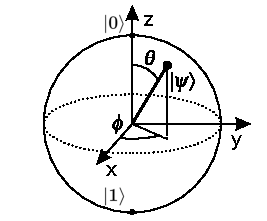
\includegraphics[width=.28\linewidth]{figures/BlochSphereCropped.pdf}
	\caption{The Bloch sphere representation. A classical bit can only be $\ket{0}$ or $\ket{1}$, whereas a qubit can occupy any point on the sphere with coordinates $\theta, \phi$. Figure adapted from \cite{Jones2012}.}
	\label{fig:BlochSphere}
\end{figure}

\subsection{Entanglement}\label{sub:Entanglement}

We will extend from 1 to 2 electrons. Now, they can be independently spin up $\ket{0}$ and down: $\ket{1}$, for a total of 4 basis states. Quantum physics teaches us this system can be in a superposition of all its basis states \cite{Nielsen2011}:

\begin{equation}\label{eq:TwoQubits}
	\ket{\psi_{2q}} = 
	\alpha_{00} \ket{00} + \alpha_{01} \ket{01} + \alpha_{10} \ket{10} + \alpha_{11} \ket{11}.
\end{equation}

Where $\ket{00}$ is a shorthand notation for both qubits being in the spin-up state, etc. In general, the size of the Hilbert space will grow as $2^N$ for $N$ qubits \cite{Henriet2020,Nielsen2011}. For $N=300$, this is already larger than the estimated amount of particles in the observable universe at some $\sim 10^{80}$. However, to access the full Hilbert space, the qubits need to be entangled. These are an inherent quantum feature, having no classical analog. One of the most instructive examples of an entangled state is 

\begin{equation}\label{eq:Entangled}
	\ket{\Phi^+} = \frac{1}{\sqrt{2}} \ket{00}+ \frac{1}{\sqrt{2}} \ket{11}
\end{equation}

This is one of the so-called Bell states \cite{Nielsen2011} and it is said to be entangled: upon measuring just one of the qubits we immediately know the state of the other qubit as well. This implies the qubits are correlated and cannot be described as a product of independent single qubits. In the operation of a quantum computer, entanglement is a crucial step during the computation stage \cite{Henriet2020}. 

\section{The NISQ Era}

Apart from controlling the quantum states of individual qubits, qubits are to be shielded from the environment, as noise from the environment can change the quantum states of the qubits.  This effect is known as decoherence \cite{DiVincenzo2000}. Decoherence errors can be corrected but this requires significant overhead in the available number of qubits and is unachievable in the near term \cite{Peres1985,Ladd2010}. Therefore, quantum computing is currently said to be in the \ac{NISQ} \cite{Preskill2018}. During the \ac{NISQ} era, the algorithms that run on quantum computers should be optimized for finite coherence times and fidelities. One algorithm proposed by \cite{Peruzzo2014} is thought to run especially well on non error-corrected hardware, so we will briefly describe its basic principle here \cite{McClean2016}. 

\subsection{The Variational Quantum Eigensolver}

The \ac{VQE} is a hybrid quantum algorithm: by making use of classical hardware it aims to reduce the number of quantum gates needed, which is advantageous on NISQ era hardware with finite coherence times \cite{McClean2016}. Essentially, \ac{VQE} tries to find approximately the ground state energy of an atom or molecule according to the variational principle \cite{Griffiths2004}, which states that the expectation value of a given Hamiltonian $\mathcal{H}$ will always be an upper bound for the ground state energy $E_g$:

\begin{equation}\label{eq:VariationalPrinciple}
	\left\langle \mathcal{H} \right\rangle = \bra{\Psi}\mathcal{H} \ket{\Psi} \geq E_g.
\end{equation}

This is equivalent to finding the eigenvalues of the matrix $\mathcal{H}$. Even for relatively simple molecules, $\mathcal{H}$ quickly becomes large and the task op diagonalizing it intractable, at least for a classical computer. In \ac{VQE}, $\mathcal{H}$ is not directly diagonalized but the Hamiltonian is prepared in a quantum co-processor or \ac{QPU} \cite{Henriet2020,Peruzzo2014}, taking advantage of the large Hilbert state of the quantum hardware. Given an ansatz $\theta$, a trial state $\ket{\Psi(\theta)}$ is prepared. The Hamiltonian is written in the form of a sum of Pauli strings: $P_{\alpha}$ with weights $h_{\alpha}$ \cite{McClean2016,Moll2018}

\begin{equation}\label{eq:PauliDecomposition}
	\mathcal{H} = \sum_{\alpha} h_{\alpha} P_{\alpha}
\end{equation}

\begin{figure}
	\centering
	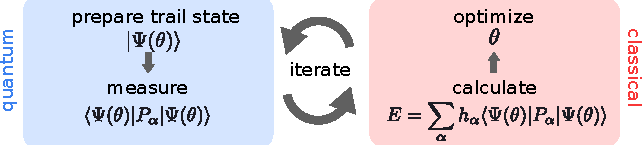
\includegraphics[width=0.75\linewidth]{figures/VQE.pdf}
	\caption{The \ac{VQE} visualized. Meant to run on a hybrid quantum computer, starting from an ansatz for the wave function it is prepared and the expectation function of its energy measured by a series of measurements on the \ac{QPU}. Next, a CPU uses a non-linear optimization to find a new ansatz that will decrease the expectation value of $\mathcal{H}$. Iterated until convergence. Figure adapted from \cite{Moll2018}}
	\label{fig:VQE}
\end{figure}

The Pauli string is essentially a tensor product of Pauli spin matrices, the definition is given in appendix \ref{ch:PauliExpectation}. Because of the decomposition in Pauli strings, estimating the various terms of the Hamiltonian $\bra{\Psi} P_{\alpha} \ket{\Psi}$ boils down to measuring populations of individual qubits, this is explained in appendix \ref{ch:PauliExpectation}. The total expectation value of the Hamiltonian is obtained by summing over contributions of the Pauli strings. This is done on classical hardware. Subsequently, a non-linear optimizer is run to minimize the energy using a new trial state, which is fed back into the \ac{QPU}. \cite{Moll2018}. The algorithm is visualized in \cref{fig:VQE}. The quantum and classical components of the algorithms feed into each other, therefore \ac{VQE} is referred to as a hybrid algorithm. 

\subsection{Hardware Implementation}

There are many options for implementing the algorithm on quantum hardware. \cite{DiVincenzo2000} formulated a list of criteria the hardware is to adhere to. Based on this, several quantum computer realizations have been proposed \cite{Ladd2010}. Examples include infrared photons \cite{Matthews2009},  trapped ions \cite{Benhelm2008,Schindler2013}, electron spins \cite{Press2008} and superconducting currents \cite{DiCarlo2009,Arute2019}. 

Another implementation is to use qubits encoded in the electronic states of neutral atoms. These atoms are assembled in arbitrary geometries using laser cooling and trapping techniques. One of those techniques is using tightly focused laser beams to trap atoms, also known as optical tweezers. This technique is thought to easily scale to a higher number of qubits by increasing the trapping laser power \cite{Henriet2020}. The atoms are held in place by optical dipole traps \cite{Chu1986}, each trap is non-deterministically loaded with single atoms \cite{Schlosser2001}. Multiple dipole traps spaced a couple of micrometers from each other are made using holography techniques \cite{Bergamini2004}. Interactions between qubits are realized using excitation to very high principle quantum numbers (Rydberg states) \cite{Levine2018,Madjarov2020}. Lastly, projections of qubit states are measured using laser induced fluorescence. An overview of the different steps in neutral atom quantum computing is shown in \cref{fig:ComputingSteps}.

\begin{figure}
	\centering
	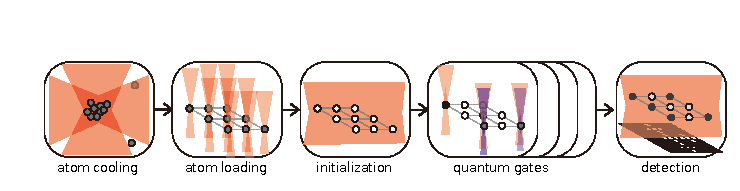
\includegraphics[width=\linewidth]{figures/ComputingSteps.pdf}
	\caption{Steps involved in running a \ac{QPU} based on neutral atoms in optical tweezers. Figure from \cite{Wu2021}.}
	\label{fig:ComputingSteps}
\end{figure}

\section{This Thesis}

In a collaboration with the \textit{Schreck} group, we aim to realize a \ac{QPU} based on strontium (Sr) atoms, which was recently shown to achieve high-fidelity quantum gates and measurements \cite{Madjarov2020}. The purpose of this thesis is to give an update of the first steps carried out in our group towards this goal. Therefore, this work is mostly about the first two steps in \cref{fig:ComputingSteps}. To to this the work is organized in the following way:

\begin{itemize}
	\setlength\itemsep{-1pt}
	\item Background information about laser cooling and trapping techniques, as well as for Sr specifically is presented in \cref{ch:coolingtrapping}. 

	\item Chapter \cref{ch:tweezer} is about focusing a laser beam to the smallest possible spot inside of a vacuum chamber, to realize an optical tweezer.

	\item Chapter \ref{ch:arrays} elaborates on how to make arrays of tweezers in arbitrary geometries by using holography techniques.

	\item Finally, in \cref{ch:implementation} we describe how to implement the setup in an ultracold experiment. Because the Sr atom source and laser system is set to arrive after this thesis was completed, we show progress towards trapping rubidium (Rb) instead, but the tweezer platform should work for Sr as well. 
\end{itemize}











\chapter{Laser Cooling and Trapping}\label{ch:coolingtrapping}In assembly, computation, and readout of single atoms, laser cooling and trapping techniques play a central role. This chapter will give some background on how this technique works, and how we intend to apply it onto strontium (Sr).
%stress difference between near-resonant regime dominated by scattering 2 level and off-resonant

\section{Magneto-Optical Trap}

The workhorse for producing clouds of ultracold atoms is the 3D \ac{MOT}. In essence, it consists of three sets of counter-propagating beams as well as a magnetic field gradient, together providing a dampening as well as a confining force. 

\subsection{Doppler Cooling}

Consider an atom with ground state $\ket{g}$ and excited state $\ket{e}$ separated by energy splitting $\hbar \omega_0$. This convention will be used for the remainder of this work. We drive a laser with omega $\omega$ that is near-resonant, but \emph{detuned} slightly from the transition by an amount $\delta$:

\begin{equation}\label{detuning}
	\delta = \omega - \omega_0
\end{equation}

It will turn out that detuning is one of the most important parameters in laser cooling. In this work we will always have $\delta <0$. Because of the Doppler effect, the atom 'sees' a slightly different light frequency depending on its velocity $v$ according to $\delta'=\delta+kv$ and the laser may become resonant: $\delta' = \omega_0$, causing the atom to absorb a photon absorbing momentum $\hbar k$ and promoting an electron to the excited state $\ket{e}$. When spontaneous emission causes the atom to fall back in a time $\tau = 1/\gamma$ where $\gamma$ is the linewidth of the transition, the electron is decayed back to the ground state, but the emitted photon is emitted in a random direction. This can be repeated many times per second at a scattering rate $\Gamma_{\text{sc}}$ \cite{Metcalf1999}

\begin{equation}\label{eq:ScatteringFrequency}
	\Gamma_{\text{sc}} = \frac{ \gamma s_0 /2}{1+s_0+\left[2(\delta+ k v)/\gamma\right]^2},
\end{equation}

where $s_0 = I/I_{sat}$ is the saturation parameter as a function of the light intensity $I$ for saturation intensity $I_{sat} = \hbar c \gamma \pi/3\lambdaup^3$ for wavelength $\lambda$ and linewidth $\gamma$. Because the absorption occurs in a fixed direction and the emission is a random event, the atom will experience a net force scattering force $F = \hbar k \Gamma_{sc}$.

\subsection{Optical Molasses}

We can reflect the laser beam using a mirror, such that the force works in both directions of the spatial coordinate. We will only consider one spatial coordinate which we will denote as $z$, but the treatment can be easily extended to 3 dimensions. The total force from both contributions from \cref{eq:ScatteringFrequency} is \cite{Kowalski2010}

\begin{equation}\label{eq:OpticalMolasses}
	F = \frac{\hbar k \gamma s_0}{2}\left\{\
	\left[1 + s_0 + 4\frac{(\delta+kv)^2}{\gamma^2}\right]^{-1}+
	\left[1 + s_0 + 4\frac{(\delta-kv)^2}{\gamma^2}\right]^{-1}
	\right\}
\end{equation}

We have plotted the result of \cref{eq:OpticalMolasses} in \cref{fig:MOTcooling} as a function of velocity in units of $\hbar / k$, such that it is dimensionless. Contributions of both beams, as well as their total force, are shown in units of $\hbar k \gamma$. Doing a series expansion to first order around $v = 0$. For $\delta<0$ we find we can linearize the force $F$ as \cite{Metcalf1999}

\begin{figure}
\centering
	\begin{subfigure}{.38\textwidth}
		\centering
		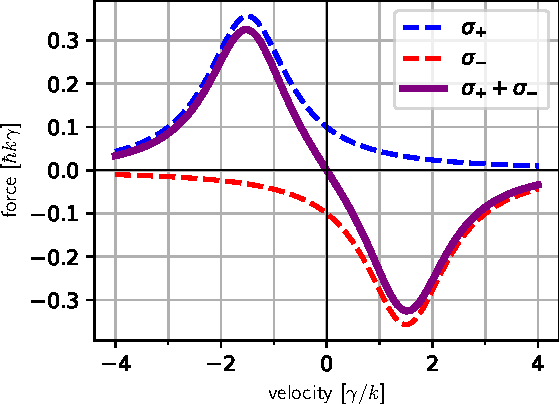
\includegraphics[width=\linewidth]{figures/MOTplot.pdf}
		\caption{}
		\label{fig:MOTcooling}
	\end{subfigure}
	\begin{subfigure}{.52\textwidth}
		\centering
		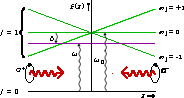
\includegraphics[width=\linewidth]{figures/OpticalMolasses.pdf}
		\caption{}
		\label{fig:MOTconcept}
	\end{subfigure}
	\caption{a) Cooling force from a magneto-optical trap. Contributions from the $F^+$, $F^-$ and the total force are shown for $\delta = -\gamma$ and $I/I_0 = 2.$ Concept of optical molasses in 1D. Atomic frequency is detuned from the atomic transition by $\delta<0$. Because of the linear magnetic field, for $z>0$, the $m_j=-1$ atoms become resonant with only $\sigma^+$ light because of selection rules, and vice versa.}
	\label{fig:MOTPlots}
\end{figure}

\begin{equation}\label{eq:ForceLinearized}
	F \sim - \hbar k^2 s_0 \frac{-2\delta/\gamma}{\left[1+s_0+(2\delta/\gamma)^2\right]^2} \equiv -\beta v
\end{equation}

Where $\beta$ is the slope of the scattering force around $v=0$. The resulting force has a dampening character on the velocity, which if applied in all 3 dimensions can cool atoms to ultracold temperatures. 

The treatment so far would suggest that this can be used to cool atoms to temperatures of absolute zero. This is not the case, as the random character of the scattering force means the atom fluctuates around the equilibrium velocity according to a Brownian motion. 
%balance betweeen cooling and recoil heating. For higher s0 it is doppler broadened by a factor 
For $\delta=-\gamma/2$, \cref{eq:ForceLinearized} ($\beta$) is at a maximum, yielding the lowest possible temperature achievable using Doppler cooling: the Doppler temperature $T_D$ \cite{Metcalf1999}

\begin{equation}\label{eq:DopplerTemperature}
	T_D = \frac{\hbar}{2k_b} \gamma.
\end{equation}

where $k_b$ is Boltzmann's constant. Apparently, this cooling limit is only dependent on the linewidth of the transition $\gamma$, apart from physical constants. This result will be used later in \cref{sec:Sr}.

\subsection{Magnetic Trapping}

Apart from cooling the atoms, we want to trap them at a specific location to increase the density of atoms. We can use the Zeeman effect for this, which tells us the atomic energy levels will be split an amount $\Delta E$ according to \cite{Griffiths2004}

\begin{equation}\label{eq:Zeeman}
	\Delta E = \mu_{\emph{B}} g_J m_j B,
\end{equation}

where $\mu_{\emph{B}}$ Bohr magneton, $g_J$ the Landé g-factor, $m_j$ is the magnetic quantum number and $B_{\text{ext}}$ the applied magnetic field. The magnetic field is tuned in such a way that it is linear in all 3 dimensions and zero at the center of the \ac{MOT} by using a set of magnetic field coils in an anti-Helmholtz configuration. Because of the Zeeman splitting, the chance of the atoms coming in resonance with the laser varies with the position from the origin according to \cite{Kowalski2010}

\begin{equation}\label{eq:DetuningFull}
	\delta' = \delta + k v - \frac{\mu'B}{\hbar}
\end{equation}

Where $\mu' = (g_e m_e-g_g m_g)\mu_B$ is the effective magnetic moment for the transition \cite{Kowalski2010}. To ensure that atoms only absorb momentum kicks in the right direction, the laser beams are circularly polarized: $\sigma^+$ from the left and $\sigma^-$ from the right. Because the sign of the Zeeman shift is dependent on the magnetic quantum number $m_j$, selection rules prescribe that atoms displayed by $z>0$ are only resonant with $\sigma^-$-light and vice versa. This is sketched in \cref{fig:MOTconcept}. Inserting \cref{eq:DetuningFull} in \cref{eq:OpticalMolasses} yields

\begin{equation}\label{eq:MOTfull}
	\frac{F}{\hbar k \gamma s_0} = \frac{1}{2}\left\{\
	\left[1 + s_0 + 4\frac{(\delta+kv+\mu'B/\hbar)^2}{\gamma^2}\right]^{-1}+
	\left[1 + s_0 + 4\frac{(\delta-kv-\mu'B/\hbar)^2}{\gamma^2}\right]^{-1}
	\right\}
\end{equation}

Expanding \cref{eq:MOTfull} around $(v,z) = (0,0)$, keeping only first order terms finally leaves us with \cite{Kowalski2010}

\begin{equation}\label{eq:ForceMOT}
	F_{\text{MOT}}(z,v) \sim -\beta v - \kappa z.
\end{equation}

Where $\beta$ is the same we found in \cref{eq:ForceLinearized} and $\kappa \equiv \mu' \beta /\hbar k \cdot \partial B/\partial z$. Apart from the dampening force, we now also have a restoring force. When applied in 3 dimensions this can be used to make clouds of ultracold atoms. 

\section{Optical Dipole Traps}\label{sec:OpticalDipoleTrap}

While magneto-optical traps are excellent for producing clouds of ultracold atoms, the constant photon scattering is unwanted during qubit operation. Therefore, after the atom cloud is cooled in the \ac{MOT}, it is typically loaded in another type of trap: the \ac{ODT}. An ODT uses far-off-resonant light. Though this means that the coupling and therefore the trapping is weaker, it has negligible scattering, which is important to maintain coherence of quantum states. We consider a radiation field $\mathbf{E}$. This field will induce a dipole moment $\mathbf{p}$ in the atom according to 
	
\begin{equation}\label{eq:DipoleMoment}
	\mathbf{p} = \alpha \mathbf{E}.
\end{equation}

Consequently, the dipole potential will interact with the electric field leading to and an interaction dipole potential $U_{\text{dip}}$ as a function of the position vector $\mathbf{r}$ \cite{Grimm2000}

\begin{equation}\label{eq:DipolePotential}
	U_{\text{dip}}(\mathbf{r}) = -\mathbf{p}\mathbf{E} = 
	-\frac{1}{2} \left\langle \mathbf{p}\mathbf{E} \right\rangle = \frac{\operatorname{Re}(\alpha)}{2\epsilon_0 c} I(\mathbf{r}),
\end{equation}

where the $\left\langle\right\rangle$ brackets denote the time average. We average over this radidly varying phase term, yielding a factor $1/2$. Furthermore we used $I(\mathbf{r}) = |\mathbf{E}(\mathbf{r})|^2/(2\epsilon_0 c)$ where $\epsilon_0$ is the electric constant. The dipole force thus scales with the in-phase part of the polarizability with the light field. An additional factor $1/2$ comes in because the dipole moment is induced and not permanent \cite{Grimm2000}. The gradient of \cref{eq:DipolePotential} gives rise to the dipole force:

\begin{equation}\label{eq:DipoleForce}
	\mathbf{F}_{\text{dip}}(\mathbf{r}) = - \frac{\operatorname{Re}(\alpha)}{2\epsilon_0c}\nabla I(\mathbf{r})
\end{equation}

The dipole force can be used to coherently trap our qubits. To maximize the dipole force \cref{eq:DipoleForce}, we have to maximize the gradient of the light intensity profile. This can be done by focussing the laser on the smallest possible spot. How we do this is explained in \cref{ch:tweezer}. The scattering rate from the ODT can be found by averaging over the derivative of the dipole moment with the electric field \cite{Grimm2000}

\begin{equation}\label{eq:ScatteringRate}
	\Gamma_{\text{sc}}(\mathbf{r}) = \frac{\left\langle \mathbf{p} \mathbf{E} \right\rangle}{\hbar \omega}
	 = \frac{\operatorname{Im}(\alpha)}{\hbar \epsilon_0 c} I(\mathbf{r}).
\end{equation}

\cref{eq:DipoleForce,eq:ScatteringRate} are general expressions for any potential. The fact that $\alpha(\omega)$ is complex means there is a phase delay between the electric field and the dipole response. The task that remains is finding the polarizability $\alpha(\omega)$. As a starting point, we will consider the electron as a (classical) damped harmonic oscillator, which is for Alkali species already fairly accurate \cite{Grimm2000}.

\subsection{Classical}

In the classical picture, we assume a classical light field, as well as a classical electron (harmonic oscillator). We can write down a general expression for the the light field propagating in the $z$-direction polarized in the $\bm{\hat{\epsilon}}$ direction perpendicular to it:

\begin{equation}\label{eq:ClassicalField}
	\mathbf{E}(z,t) = \mathbf{E}_0 \cos{(k z - \omega t)} 	\bm{\hat{\epsilon}}
\end{equation}
	 
The electron is modeled as a damped harmonic oscillator (Lorentz oscillator). Integrating the equation of motion for the electron, assuming a dipole moment $\mathbf{p} = e \mathbf{r}$ where $r$ is the position yields after equating to \cref{eq:DipoleMoment} for the polarizability \cite{Grimm2000}

\begin{equation}\label{eq:LorentzOscillator}
	\alpha(\omega)=6 \pi \epsilon_{0} c^{3} \frac{\Gamma / \omega_{0}^{2}}{\omega_{0}^{2}-\omega^{2}-\mathrm{i}\omega^3\Gamma/\omega_0^2}
\end{equation},

Where $\Gamma$ is the on-resonant damping rate in terms of the electron mass $m_e$. 

\begin{equation}\label{eq:ResonantDampingRate}
	\Gamma = \frac{e^2 \omega_0^2}{6\pi \epsilon_0 m_e c^3}
\end{equation}

Inserting \cref{eq:LorentzOscillator} in \cref{eq:DipolePotential,eq:ScatteringRate} yields, after assuming $\delta \ll \omega, \Gamma \ll \omega$

\begin{equation}\label{eq:DipoleClassicalResult} 
	U_{\text{dip}}(\mathbf{r}) = 
	\frac{3\pi c^2}{2\omega_0^3}\frac{\Gamma}{\delta} I(\mathbf{r}),
	\quad
	\Gamma_{\text{sc}}(\mathbf{r}) = 
	\frac{3\pi c^2}{2\hbar\omega_0^3}\left(\frac{\Gamma}{\delta}\right)^2 I(\mathbf{r})
\end{equation}

From \cref{eq:DipoleClassicalResult} the relation these two quantities is $\hbar \Gamma_{sc} =\Gamma U_{\text{dip}}/\delta$. Thus, to keep scattering events to a minimum a large detuning should be used. To still have sufficiently deep traps, high light intensities are used. 


\subsection{Semi-Classical}

In the semi-classical picture, we consider the same classical light field \cref{eq:ClassicalField}, but consider an atom with quantized energy levels. We will consider a two-level atom with eigenstates $\ket{g}$ (ground) with energy $\hbar \omega_g$ and $\ket{e}$ (excited) with $\hbar \omega_e$, see \cref{fig:2LevelAtom}. Then the atomic Hamiltonian in this basis reduces to \cite{Loudon2000}

\begin{figure}
	\centering
	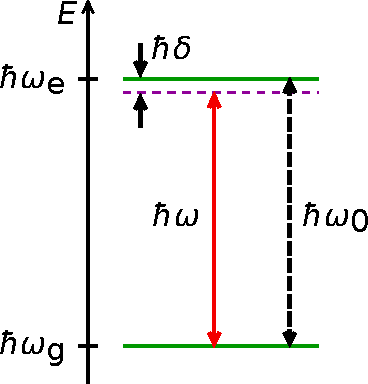
\includegraphics[height=4.1cm]{figures/2LevelAtom.pdf}
	\caption{Energy level scheme for the 2-level case. The two energies are split by $\omega_e - \omega_g = \omega_0$. The detuning is $\delta = \omega-\omega_0<0$ is shown as well.}
	\label{fig:2LevelAtom}
\end{figure}

\begin{equation}\label{eq:AtomHamiltonianMain}
	\mathcal{H}_A = \hbar \omega_g \ket{g}\bra{g} + \hbar \omega_e \ket{e}\bra{e}
\end{equation}

The radiation field is modeled as a time-dependent perturbation such that the total Hamiltonian is \cite{Leeuwen2017}

\begin{equation}\label{eq:PerturbationMain}
	\mathcal{H} = \mathcal{H}_A + \mathcal{H}_{I}(t),
\end{equation}

We can write down the combined wave function in the basis of the unperturbed eigenstates, its time evolution given by

\begin{equation}\label{eq:TwoLevelMain}
	\ket{\psi(t)} = c_g(t) e^{-i \omega_g t} \ket{g} + c_e(t) e^{-i \omega_e t} \ket{e}.
\end{equation}

In appendix \ref{ch:LightMatter} the Schrodinger equation is solved for the 2-level atom using the dipole approximation as well as the \acf*{RWA}. The following matrix equation is derived for the 2 level atom (\cref{fig:2LevelAtom}) \cite{Foot2005}

\begin{equation}\label{eq:MatrixEvolution}
	i \hbar \begin{pmatrix}
		\dot{c}_g \\ 
		\dot{c}e
	\end{pmatrix}
	= \frac{\hbar}{2} \begin{pmatrix}
		\delta & \Omega \\ \Omega^* & -\delta 
	\end{pmatrix} 
	\begin{pmatrix}
		c_g \\ c_e,
	\end{pmatrix}
\end{equation}.

where the coupling between the atomic eigenstates and the radiation field is described by the Rabi frequency \cite{Metcalf1999}:

\begin{equation}\label{eq:RabiFrequencyMain}
	\Omega \equiv \frac{e E_0}{\hbar} \bra{g}\mathbf{r}\ket{e}.
\end{equation}

The Hamiltonian of \cref{eq:MatrixEvolution} has eigenvalues 

\begin{equation}\label{eq:EigenValues}
	E_{\pm} = \pm
	\frac{\hbar}{2} \sqrt{\Omega^2+\delta^2}.
\end{equation}

Assuming $|\delta| \gg \Omega$, the eigenenergies are thus 

\begin{equation}\label{eq:SemiClassicalEigenvalues}
	E_g \sim  \frac{\hbar \delta}{2} +\frac{\hbar \Omega^2}{4 \delta}, \quad
	E_e \sim -\frac{\hbar \delta}{2} -\frac{\hbar \Omega^2}{4 \delta}
\end{equation}

When turning on the laser, the energies are thus shifted by an amount $\Delta E = E(\Omega)-E(\Omega=0)$. This is called the light shift or AC Stark shift \cite{Metcalf1999}, sketched in \cref{fig:DipoleForce}.

\begin{figure}
    \centering
	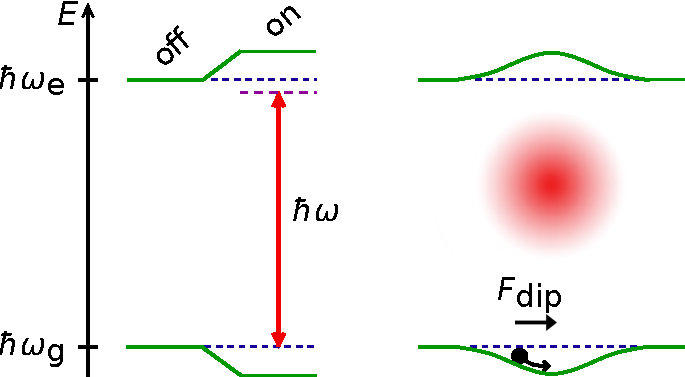
\includegraphics[height=3.8cm]{figures/LightShift.pdf}
	\caption{Light shift when the off-resonant laser is turned on, as well as the spatially varying light shift for a laser beam profile for $\delta<0$. Figure not to scale.}
	\label{fig:DipoleForce}
\end{figure}

\begin{equation}\label{eq:Stark}
	\Delta E_{e,g} \sim \pm \frac{\hbar \Omega^2}{4 \delta}.
\end{equation}

The light shift is proportional to the light intensity over the detuning: $\Omega^2 / \delta \propto I / \delta$, which we already found for the classical treatment in \cref{eq:DipoleClassicalResult}. This behavior of \cref{eq:Stark} is shown in \cref{fig:DipoleForce}. Because the field is off-resonant, atoms only occupy the ground state. For $\delta <0$ ('red detuned'), the ground state light state is negative. To calculate the new eigenstates, we repeat the treatment for a quantized light field. This is known as the dressed atom picture.

\subsection{Dressed Atom Picture}\label{sec:DressedApproach}

To calculate the new shifted eigenstates, the full Hamiltonian has to be considered, included a quantized light field with Hamiltonian $\mathcal{H}_L$ \cite{Dalibard1985}

\begin{equation}
	\mathcal{H} = \mathcal{H}_A + \mathcal{H}_L + \mathcal{H}_I(t)
\end{equation}

where the light field has eigenenergies separated by the photon energy and eigenstates of $n$ photons: $\ket{n}$ \cite{Vredenbregt2020}

\begin{equation}\label{eq:RadiationModes}
	\mathcal{H}_L = \sum_n \hbar \omega \left(n+\frac{1}{2}\right) \ket{n}\bra{n}
\end{equation}

The eigenmodes of the light field can only couple to one energy pair of the $\mathcal{H}_A + \mathcal{H}_I$ part, such that the Hamiltonian can be written down as a direct product of 2 x 2-matrix Hamiltonians \cite{Vredenbregt2020,Hussin2005} $\mathcal{H}_n$:

\begin{equation}\label{eq:CunningsHamiltonian}
    \mathcal{H}_n = \hbar 
    \begin{pmatrix}
        (n + 1)\omega -\omega_0 / 2                     & -\frac{1}{2}\sqrt{\Omega^2+\delta^2(n+1)} \\
        -\frac{1}{2}\sqrt{\Omega^2 + \delta^2(n+1)}  & n\omega + \omega_0/2
    \end{pmatrix}
\end{equation}

This is known as the Jaynes-Cummings Hamiltonian, which is one of the few problems in quantum optics analytically solvable. It has eigenvalues \cite{Hussin2005}

\begin{equation}\label{eq:CunningsEigenvalues}
    E_{\pm} = \hbar\omega\left(n+\frac{1}{2}\right) \pm \frac{\hbar}{2} \sqrt{\delta^2 + \Omega^2(n+1)}.
\end{equation}

Note the similarity to \cref{eq:SemiClassicalEigenvalues}. From \cref{eq:CunningsEigenvalues} the new eigenstates can be found to be \cite{Hussin2005}

\begin{subequations}\label{eq:CummingsEigenstates}
    \begin{align}
        \ket{+,n} &= \cos{({\theta_n}/2)} \ket{n+1,g} -\sin{(\theta_n/2)} \ket{n,e}, \\
        \ket{-,n} &= \sin{(\theta_n/2)}\ket{n+1,g} + \cos{(\theta_n/2)} \ket{n,e}.
    \end{align}
\end{subequations}

Which are sketched in \cref{fig:DipoleForce} as well. In \cref{eq:CummingsEigenstates} the mixing angle $\theta_n$ for $n$ photons in the system is

\begin{equation}
    \theta_n = \arctan{\left(
        \frac{\Omega\sqrt{n+1}}{\delta}
    \right)}
\end{equation}

Here, \cref{eq:CummingsEigenstates} are known as the \emph{dressed} states. The \emph{bare} atomic states in \cref{fig:2LevelAtom} are shifted by the light shift because the light field energy is admixed with the atomic eigenstates, leading to the new mixed (dressed) eigenstates of \cref{eq:CummingsEigenstates}. The bevavior pictured in \cref{fig:DipoleForce} still applies, but if the eigenenergies of the light field are included, the splitted energies of \cref{fig:DipoleForce} are situated along an infinite ladder of photon energies. This is presented in \cref{fig:DressedStatePicture}. The light space eigenenergies \cref{eq:RadiationModes}, spaced by $\hbar \omega$ is superimposed on the light shift eigenenergies. 

\begin{figure}
    \centering
    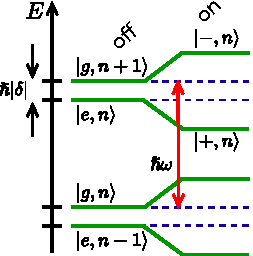
\includegraphics[width=0.31\linewidth]{figures/DressedStates.pdf}
    \caption{Dressed States. The same shift as shown in \cref{fig:DipoleForce} is shown, superimposed on the  eigenenergies spaced by $\hbar \omega$. Figue not to scale. }
    \label{fig:DressedStatePicture}
\end{figure}


\section{Strontium}\label{sec:Sr}

Historically, people started laser cooling experimentation on group 1 or alkali atoms (Na, Rb, Cs). Because they only have one valence electron, the level structure is relatively straightforward. Also, diode lasers are available for their transition frequencies. In this work, trapping of \textsuperscript{85}Rb (an alkali) is described in \cref{ch:implementation}.

However, also group 2 atoms, also called alkali-earth (and similar atoms like Yb) are possible candidates. Because of their two valence electrons, the level structure is much more complicated, making laser cooling harder, but possibly also opening up new possibilities. The element we wish to use for our new machine in Eindhoven is Sr. For more extensive coverage of Sr, the reader is referred to \cite{Stellmer2013}. Three of them are bosonic, with ${}^{88}$Sr being the most abundant at $\sim82.6\%$. There is one stable fermionic isotope: ${}^{87}$Sr has a nuclear spin of $I=9/2$ and an abundance of $\sim7.0\%$ \cite{Coursey1999}. Initially, we plan to run the machine in Eindhoven on \textsuperscript{88}Sr. Because of the lack of hyperfine structure, this isotype is a bit easier to work with, but in principle, one can use all isotopes in the same machine as the energy splitting between the isotopes is in the MHz regime, easily covered by AODs and EOMs \cite{Stellmer2013}.

\subsection{Relevant Transitions}

A simplified version of the level diagram of \textsuperscript{88}Sr is shown in \cref{fig:SrLevel}. The notation is $(n_1l_1 n_2l_2)^{2S+1}L_J$ where $n_{1,2}$ is the principal and $l_{1,2} = s, p, d, \ldots$ the azimuthal quantum number. Furthermore $S$, $L$ and $J$ are the total spin, orbital angular momentum, and total angular momentum respectively \cite{Cowan1981}.  This level scheme shows 6 out of 7 lasers to be used in this experiment. 

\begin{itemize}
	\item 461 nm. Broad transition, meaning a strong scattering force (\cref{eq:ScatteringFrequency} and high aborption-emmision cycling frequency. This is useful to slow down the hot atomic beam coming from the oven, as well as catching the atoms in a so-called blue \ac{MOT} with 'hot' temperatures of $\sim$ 1 mK.)
	
	\item 689 nm. Being much narrower than the blue transition, its Doppler temperature \cref{eq:DopplerTemperature} is much lower at $179$ nK, although in practice cooling is limited by the recoil limit to some $\sim 1$ $\mu$K \cite{Stellmer2013,Boyd2007}.
	
	\item 698 nm. The ultra-narrow clock transition ($\gamma = 1$ mHz). Used in atomic clocks because of its spectroscopic accuracy \cite{Bloom2014}. It will turn out that this feature can be put to good use in quantum computers as well, and we will use it to coherently 'drive' the qubits between the qubit basis states using this clock transition. More about this in \cref{sec:QubitScheme}
	
	\item 679, 688, and 707 nm. All repump lasers. 707 and 688 are used to cycle back atoms from ending up in ${}^3P_2$ from the decay channel shown by the grey dotted line in \cref{fig:SrLevel}. 679 is used to prevent repump leaks to ${}^3P_0$ \cite{Stellmer2013,Xu2003}.
\end{itemize}

There will also be a 813 nm laser used for the dipole trapping. This is also the most powerful laser, as it determines the limit of optical dipole traps (optical tweezers) one can make. More about this transition in \cref{sec:Magic}.

\begin{figure}
	\centering
	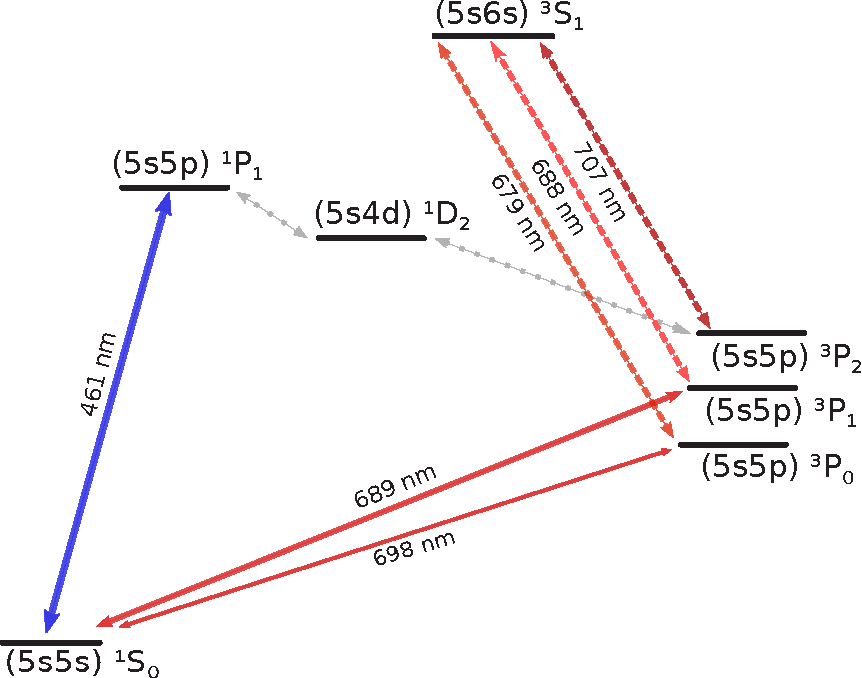
\includegraphics[width=0.51\linewidth]{figures/SrLevel.pdf}
	\caption{Simplified level scheme for \textsuperscript{88}Sr. Shown: blue transition for initial slowing and cooling. Narrower 689 nm transition of the red \ac{MOT}, and the \textsuperscript{1}S\textsubscript{0} - \textsuperscript{3}P\textsubscript{0} clock transition, which we will be used to drive the qubits. To increase density and trap lifetime 3 repump lasers are used. Not shown: 813 nm dipole trapping laser because it is driven far-off-resonant. Energies not to scale. Figure made by Ivo Knottnerus.}
	\label{fig:SrLevel}
\end{figure}

\subsection{Laser Cooling and Trapping of Sr}

Because the melting temperature of Sr is $777$ ${}^{\circ}$C, to get any relevant vapor pressure, the Sr is heated in an oven after which it sublimates. To obtain a small atomic beam divergence, the atoms are directed through a bundle of high aspect ratio capillary tubes \cite{Stellmer2013}. 

Because of the oven, the atoms are moving way too fast to be efficiently captured by the MOT. Therefore, they are slowed by a Zeeman slower. This machine uses a similar design used in the optical molasses technique, only the slowing beam is only opposing the atomic beam and not traveling along with it. A spatially varying magnetic field ensures a wide range of velocities is at some point resonant with the laser according to \cref{eq:DetuningFull}. 

Depending on the length of the Zeeman slower, only a fraction of the atoms will be slowed. To separate the hot from the cool atoms (the former are unwanted in a vacuum chamber) a deflection stage is used. The blue transition of Sr is used for this stage because of the strong scattering force. The Zeeman slowing and deflection stage is explained more elaborately in the thesis of Rik van Herk \cite{Herk2022}.

After the deflection stage, the atomic beam enters a glass cell. The advantage of using a glass cell is that it allows for the maximum amount of optical axis. To allow for longer trap survival times, the glass cell has \ac{UHV} which is separated from the stages preceding it by a differential pumping stage. 

\begin{figure}
	\centering
	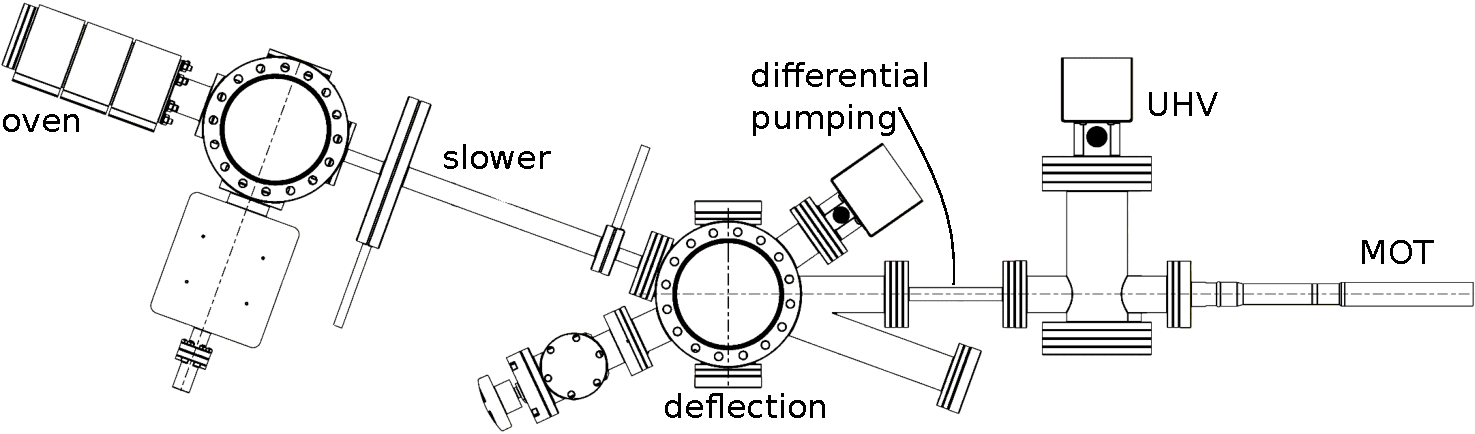
\includegraphics[width=0.8\linewidth]{figures/SrLoading.pdf}
	\caption{Sketch of the vacuum atom source design and vacuum chambers. Starting from the oven, the atomic beam traverses a Zeeman slower, deflection stage, and differential pumping stage before ending in the glass cell (MOT, right). The author did not contribute to this design. Figure by Patrick de Laat.}
	\label{fig:SrLoading}
\end{figure}

\subsection{Strontium as a Qubit}\label{sec:QubitScheme}

One of the main reasons we want to use strontium atoms for the quantum processing unit is the ${}^3P_0$ state and its very long lifetime. The clock transition is forbidden according to selection rules and only opens up after applying a magnetic field for the \textsuperscript{88}Sr isotope. Therefore,  ${}^3P_0$ is called meta-stable and can be considered a ground state on the time scale of the operation of a quantum processing unit. ${}^1S_0$ is the other clock state. Therefore, we effectily have two ground states and we can denote our qubit states as $\ket{g_1}$ and $\ket{g_2}$ (the clock states) as

\begin{equation}\label{eq:QubitManifold}
	\big\{\ket{0},\ket{1}\big\} = 
	\left\{
		\ket{{}^1S_0}, \ket{{}^3P_0} 
	\right\} = 
	\left\{ 
	    \ket{g_1}, \ket{g_2}
	\right\}.
\end{equation}

So we have two long-lifetime states connected by an extremely narrow linewidth coupling between them, that can be used to drive the qubits on the Bloch spheres. To entangle the qubits, Rydberg dressing can be used \cite{Wu2021} where a small part of a Rydberg state $\ket{r}$ is admixed in the higher energy ground state:

\begin{equation}\label{eq:RydbergDressing}
	\ket{\psi} \sim \ket{g_2} + \epsilon \ket{r}
\end{equation}

The amount of dressing is tuned by the (small) dressing parameter $\epsilon \propto \Omega / 2\delta$ where $\Omega$ is the Rabi frequency of the laser and $\delta$ the usual detuning. A Rydberg state is an electronic state with a very high principal quantum number $n$. Rydberg atoms are physically larger, as the electron orbit radius scales $\propto n^2$ \cite{Gallagher1994}. As a result of these exaggerated electron orbit sizes, neighboring atoms can 'feel' each other. For example, the van der Waals interaction coefficient scales as $\propto n^{11}$ \cite{Gallagher1994}. 

Other qubit implementations than the one above are possible as well. For example, \cite{Barnes2021} uses the fermionic ${}^{87}$Sr and maps the qubit states onto the nuclear spin states $\ket{{}^1S_0, F=9/2, m_F = -9/2}$ and $\ket{{}^1S_0, F=9/2, m_F = -7/2}$.

\subsubsection*{Magic Trapping of Strontium}\label{sec:Magic}

\begin{figure}
    \centering
    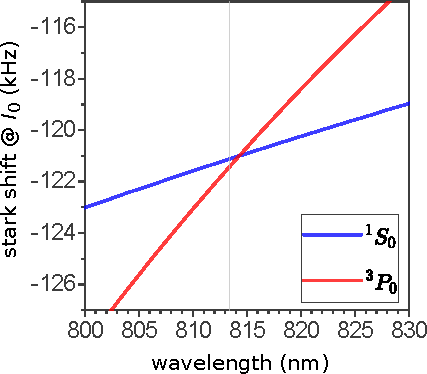
\includegraphics[width=0.38\linewidth]{figures/Magic.pdf}
    \caption{Atomic polarizabilities of ${}^1S_0$ and ${}^3P_0$ showing a magic crossing around 813 nm. Grey line: experimental result. Figure adapted from \cite{Boyd2007}.} 
    \label{fig:BoydMagic}
\end{figure}

To use the states in \cref{eq:QubitManifold} in a quantum processing unit, they should both be trapped. Because the trapping potential is wavelength dependent, in general, the trapping potential will not be the same for both qubit states when using the same trapping wavelength (\cref{eq:DipoleForce}: $U_{\text{dip}} \propto - \operatorname{Re}\{\alpha(\omega)\} I(\mathbf{r})$, meaning that the transition frequency between the qubit states would change as a function of the position within the potential which is unfavorable. Instead, \cite{Katori2003} proposed to use a wavelength where the polarizability $\alpha(\omega)$ or $\alpha(\lambdaup)$ is identical for both clock states as measured by \cite{Takamoto2005,Jun2008}.

Calculating this \textit{magic} crossing point of \cref{eq:MagicCrossing} is outside the scope of this thesis, but we will show the final result as found by \cite{Boyd2007} in \cref{fig:BoydMagic}. The reader is referred to \cite{Madjarov2020,Boyd2007} for more information. Plotting the polarizability for both clock states as a function of wavelength and one findes a magic crossing point around 813 nm. By trapping both qubit states in the same potential, one can coherently drive the qubits to any point on the Bloch spheres. 

Both qubit states coupled far-off-resonantly to a different excited states using this same magic potential. The excited states used can be found in \cref{fig:SrLevel}. That figure is one again plotted in \cref{fig:2LevelTweezer}, where the two different dipole trap schemes are highlighted.

\begin{equation}\label{eq:MagicCrossing}
    \operatorname{Re}\left\{\alpha(\lambdaup-\lambdaup_{\ket{g_1})})\right\} = 
    \operatorname{Re}\left\{\alpha(\lambdaup-\lambdaup_{\ket{g_2})})\right\}
\end{equation}

\begin{figure}
    \centering
    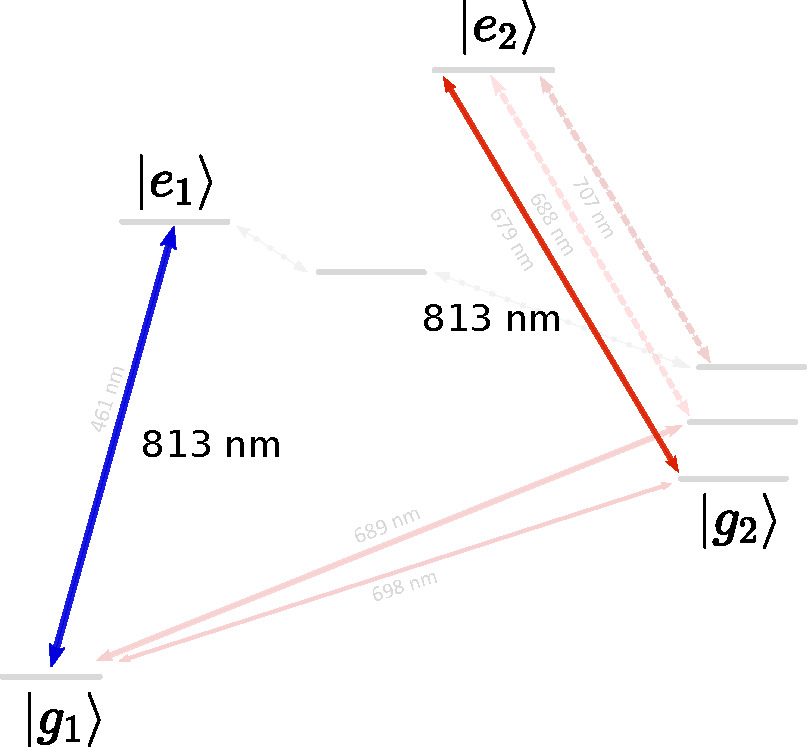
\includegraphics[width=.38\linewidth]{figures/2groundTweezer.pdf}
    \caption{Both clock states, here denoted $\ket{g_1}, \ket{g_2}$ are coupled to a different excited state: $\ket{e_1}, \ket{e_2}$ using the same trapping laser at 813 nm.}
    \label{fig:2LevelTweezer}
\end{figure}



	


\chapter{Making Optical Tweezers}\label{ch:tweezer}%We will make our quantum array out of neutral strontium atoms. The tool to cool, trap and move these atoms is light. We need individual control for this. In 2001, a group from Paris showed for the first time, that if you tune your tweezer in the right way, it's possible to trap single atoms.         


 
\section{High NA objective}

In order to trap single atoms, we need to make the smallest possible spot size, the diffraction-limited spot. Fourier optics tells us that in order to make the smallest possible spot, we want to focus the light using the largest possible cone of light, so we need high NA. Apart from high NA we also need ultralong working distance, because the lens will be positioned outside of the vacuum. 

We chose the G Plan Apo 50X microscope objective from Mitutoyo. It has a fairly high NA of 0.5 and is corrected for spherical aberrations as a result of imaging through a 3.5 mm glass plate, which we will use for our vacuum. The exact glass material is not specified but we have assumed it to be N-KB7. It is designed for a finite conjugate and has a back aperture of 4 mm. We will now estimate how we use this objective in our setup. 

\subsection{Intermezzo Fourier Optics}

As we use the objective to make a tweezer, light is impinging on its back aperture. We call its complex amplitude $U(x',y')$ and define the aperture at $z = 0$ on the optical axis. After the aperture, light will show diffraction. An elegant description is provided by scalar diffraction theory. We will not repeat a full derivation here but we can refer the reader to \cite{Goodman2005}.Consider the Fresnel diffracion integral in cartesian coordinates. After the aperture, the complex amplitude $U$ distribution is:

\begin{equation}\label{FresnelDiffraction}
    U(x,y,z) = 
    \frac{e^{ikz}}{i \lambda z} \iint_{-\infty}^{\infty} U(x',y',0) \exp{\frac{ik}{2z}} \exp{\left[(x-x')^2+(y-y')^2\right]} dx'dy'.
\end{equation}

In \cref{FresnelDiffraction}, $\lambda$ is the wavelength, $k=2\pi/\lambda$ the wavenumber. In this thesis, we are usually not immediately interested in describing the light in the the near field of the aperture, but in the far-field. More formally, the following needs to apply:

\begin{equation}\label{FraunhoferCriterion}
    z \gg k R^2/2,
\end{equation}

where $R$ is the maximum distance from the aperture to the optical axis. While this criterion is in practice not met, it does hold in the focal point of a lens, because a lens projects an image in infinity to its focal length $f$. Inserting \cref{FraunhoferCriterion} in \cref{FraunhoferDiffraction} yields:

\begin{equation}\label{FraunhoferDiffraction}
    U(x, y, z)=\frac{e^{i k z} e^{i k\left(x^{2}+y^{2}\right)/2}}{i \lambda z} \iint_{-\infty}^{\infty} U(x', y') \exp \left[\frac{-ik}{z}(x x'+y y')\right] dx' dy'
\end{equation}. 

We recognize in \cref{FraunhoferDiffraction} the spatial Fourier transform, in both $x$ and $y$ with respectively the frequencies $f_x = x/\lambda z$ and $f_y = y/\lambda z$. \cref{FraunhoferDiffraction} is the Fraunhofer diffraction integral, it will be used later in this work as well. Returning back to our aperture, we are concerned with a circular aperture so a switch to cylindrical coordinates seems natural. Ignoring the phase factor in front of the integral:

\begin{equation}\label{FraunhoferRTheta}
    U(r,\theta, z) \propto \iint U(r') \exp{(\frac{- i k rr'}{z})} \exp{\left(\cos{(\theta-\theta')}\right)} r'dr'd\theta'.
\end{equation}

Using the integral definition of the Bessel function of the first kind\footnote{$J_0(x) = \frac{1}{2\pi} \int_0^{2\pi} \exp{(i x \cos{\alpha})} d\alpha$} we write \cref{FraunhoferRTheta} as 

\begin{equation}\label{FourierBessel}
    U(r,z) \propto 2\pi \int_0^{\infty} U(r') J_0\left( \frac{k r r'}{z}\right) r'dr'
\end{equation}

\cref{FourierBessel} is the Fourier-Bessel or Hankel transform. 

\subsection{Circular aperture}

Returning to initial problem: we send a Gaussian beam with width $w_i$ through an aperture of radius $R$ and are interested in what happens in the focal plane of a lens $z\approx f$

\begin{equation}\label{FourierBesselAperture}
    U(r) \propto \int_0^R e^{-r'^2/w_i^2} J_0\left(\frac{k r r'}{f}\right)r'dr'
\end{equation}

This integral has no analytical solution. We can however find an expression for the power transmission of a Gaussian beam with width $w_i$ sent through a circular aperture with radius $R$, the fraction of power transmitted issue

\begin{equation}\label{FracPowerCircular}
    P/P_0 = 1 - e^{-w_i^2/R^2}
\end{equation}

We follow \cite{Madjarov2021} and look at two extreme cases for \cref{FourierBesselAperture,FracPowerCircular}

\begin{enumerate}
    \item $w_i \gg R$. \cref{FracPowerCircular} tells us we lose almost all of our power. The aperture function can be approximated by a plane wave and dropping the exponential term in \cref{FourierBesselAperture} we find
    \begin{equation}\label{Airy}
        U(r) \propto \frac{f}{k r} J_1\left(\frac{k r R}{f}\right)
    \end{equation}
    which is the equation for an Airy pattern. It is the smallest feature a lens can produce. 

    \item $w_i \ll R$. The waist is much smaller than the aperture, according to \cref{FracPowerCircular} we have maximum power efficiency. We let the integration boundary run to infinity and using a Hankel tranform pair\footnote{$F_0(k) = \int_0^{\infty} e^{-1/2 a^2 r^2} J_0(k r)r dr = \frac{1}{a^2} e^{-\frac{k^2}{2a^2}}$} find 
        \begin{equation}
        U(r) \propto \frac{w_i^2}{2} \exp{\left(\frac{-k^2w_i^2 r^2}{2f^2}\right)}.
    \end{equation}
    The result is a Gaussian, but with a modified waist of $\lambdaup f / \pi w_0$.  The result is similar to Gaussian apodization, where the size lobes of the Airy function are gone. 
\end{enumerate}

\section{Tweezer potential}

Because we are interested mostly in what happens near the deepest point of the trap, we model the optical dipole trap as a gaussian with a maximum trap depth $-U_0$, waist $w_0$ and Rayleigh range $z_R$ to find 

\begin{equation}\label{GaussianPotential}
    I(r,z)=\frac{-I_{0}}{1+z^{2} / z_{R}^{2}} \exp \left(\frac{-2 r^{2}}{w_{0}^{2}\left(1+z^{2} / z_{R}^{2}\right)}\right)
\end{equation}

We can discuss the two extreme cases again:

\begin{enumerate}
    \item For the case $w_i \gg R$, the power transmission will be low and therefore also the trap depth $-U_0$.
    \item For $w_i \ll R$, the waist of the resulting Gaussian in radial and longitudal directions $w_0$ and $z_R$ will increase, which is undesired. Because the total amount of power in the trap is fixed, because of normalization the trap depth is lower as well. 
\end{enumerate}

It is clear that the optimum is somewhere in between these two extreme cases.  

The atoms will spend most of their time in the bottom of the tweezer. \cref{GaussianPotential} can be tailorexpanded in around the center of the tweezer, or $(r,z) = (0,0)$.

\begin{equation}\label{TaylorGaussianPotential}
    I(r,z) \approx I_0 \left(1 - \frac{2r^2}{w_0^2} - \frac{2z^2}{z_R^2}\right) \quad \text{at} \quad (r,z) = (0,0)
\end{equation}

For a potential of the form \cref{TaylorGaussianPotential} we know the frequencies: we can define the radial and longitudinal trap frequencies $\omega_r = 2\left(U_0/m w_0^2\right)^{1/2}$ and $\omega_z= \left(2 U_0/m z_R^2\right)^{1/2}$. Because we want a narrow and deep tweezer, the higher the trap frequency the better. 

The optimum trap frequency was computed numerically by \cite{Madjarov2021} and was found to be $w_i \approx R$. We will apply this result experimentally. 


\section{Point Spread Function and Diffraction Limit}

Because of the wave nature, we cannot focus a laser beam to an infinitely small spot. The smallest possible feature our high NA objective can produce is the point spread function (PSF), which we have seen is the result of illuminating the objective with a plane wave. Using \cref{Airy} we find for the intensity of the PSF around the focused beam waist:

\begin{equation}\label{AiryIntensity}
    I(r) \propto \left[\frac{J_1(krR/f)}{krR/f} \right]^2
\end{equation}

Solving for the first minimum of \cref{AiryIntensity}, we will call this radius $d$:

\begin{equation}\label{Abbe}
    d = 0.61 \frac{\lambdaup}{\text{NA}}
\end{equation}

This result is known as the Abbe limit \cite{Hecht2002} and is the reason we want to use an objective with the highest possible NA, it is Because we will not be illuminating the objective with a plane wave, but with a gaussian with a similar waist as the aperture radius, we will recover a pattern between a Gaussian and an Airy disk. It will turn out the pattern can be fit extremely well by a Gaussian ($R^2 > 0.99$). Fitting a Gaussian to an Airy disk, we find for the waist

\begin{equation}\label{GaussianAiryFit}
    w = 0.42 \frac{\lambdaup}{\text{NA}}
\end{equation}
 
Thus, when we fit a Gaussian to an Airy pattern, we can find the diffracion-limited waist from \cref{Abbe} as $w \approx 0.69 d$. Because we will use $\lambdaup = 780$ nm and $\text{NA}=0.5$ our diffraction-limited waist is $w = 655$ nm. If our waist is at this limit, we say the system is diffraction-limited, that is limited by the wave nature of light and not by aberrations or imperfections in the system. 


\section{Measuring the Tweezer potential}

We would like to measure tweezer potential of our high NA objective. We could use the objective to look at a pinhole and record its point spread function. However, in practice we don not send a plane wave but a Gaussian beam through the objective. As a result of this, two things are different \cite{Sortais2007}

\begin{itemize}
    \item As a result of apodization, the Airy rings will be damped. 
    \item The tweezer waist will be slightly broader: $\approx 9\%$.
\end{itemize}

In order to experimentally determine these effects, we send a Gaussian beam with a waist equal to the aperture radius through the microscope objective. We follow \cite{Baumgaertner2017}: we use another microscope objective to look into the tweezer waist of the Mitutoyo. But in order to avoid further convolution with the point spread function of the second objective, we use a higher NA for the second objective \footnote{Newport M-60X 0.85 NA objective}. Because there is no glass cell, this objective does not need ultra-long working distance so this higher NA is no problem. In order to record the 3D PSF, the tweezer is moved using a picomotor attenuator. 

\subsection{Calibration Imaging System}

The magnification of the Newport objective of 60X is only specified when used in a microscope with standard tube length distance, because it is finite conjugate corrected. Because our CCD is not exactly at the distance where normally the eyepiece of the microscope would be, we have to calibrate its magnification. We do this using a high resolution target \footnote{Edmund Optics high resolution microscope target.} 

We illuminate the target with an incoherent light source (LED) because the laser would cause interference from the different lines. We neglect the slightly different focus point from the Newport objective for our laser frequency compared to white light. 

\begin{figure}
    \centering
    \includegraphics[width = 2.5in]{figures/linespacing.pdf}
    \caption{Image from the resolution target illuminated showing lines spaced by 45 lines per mm.}
    \label{fig:resolutionTarget}
\end{figure}

To detect the edges in \cref{fig:resolutionTarget}, we use an edge detection algorithm script that averages over all vertical pixels, blurs using a Gaussian to surpress noise and computes the derivative. When the derivative surpasses a set threshhold we define it as an edge. The magnification was found to be $(50.3\pm0.5)$X. This is smaller than the specified 60X, which we attribute to an incorrect tube length distance. 

\subsection{Picomotor Attenuators}

The target was also used to calibrate the picomotor attenuator. We measured over the maximum available amount of lines of similar spacing of 5 using 4000 picomotor steps, and correcting for the shift in camera found a step size of $20.3\pm0.1$ nm, which matched exactly with the specifications of the piezo-attenuator for the given load. This result will be used in the 3D scanning of the tweezers. 

The stage we used is 8081-M 5-axis motorized tilt aligner from Newport. There is no reason here to use a 5-axis stage because we only need translation in one direction, but we will use this stage later to mount the objective in the final setup. To drive this stage, we used a set of Newport 8742 controllers in daisy-chain configuration. 


\section{Gaussian Beams}\label{sec:GaussianBeams}

Optical tweezer are in essence tightly focused laser beams. We will briefly revisit the description of the commonly used laser beam because it is used throughout this work. Starting from Maxwell equations, one can derive under paraxial approximation a description of the transverse electromagnetic mode (TEM\textsubscript{00}) \cite{Leeuwen2017} for the electric field $E$. This Gaussian beam is most conveniently written down in cylindrical coordinates $\{r,z\}$:

\begin{equation}\label{GaussianBeam}
	E(r,z) = \frac{w_0}{w(z)} \exp{\left(\frac{-r^2}{w^2(z)}\right)} \exp{\left[-ikz-i\frac{kr^2}{2R(z)} - i\psi(z)\right]},
\end{equation}

with parameters

\begin{equation}
	k = \frac{2\pi}{\lambdaup}, \quad 
	w(z) = \sqrt{w_0 + \frac{z^2}{z_R^2}}, \quad \text{and} \quad
	R(z) = z \left(1 + \frac{z^2}{z_R^2}\right).
\end{equation}

Respectively, the wave number in terms of the wavelength $\lambdaup$, the beam waist, the radius where the field drops $1/e$ in terms of $w(z)\equiv w_0$ and $R(z)$ is the wavefront curvature. Finally $\psi(z)$ is an extra phase term originating from the curvature of the wavefront known as the Gouy phase. We find the intensity of the Gaussian beam by taking the absolute value squared:

\begin{equation}\label{GaussianBeamIntensity}
	I(r,z) = I_0 \frac{w_0^2}{w^2(z)} \exp{\left(\frac{-2r^2}{w^2(z)}\right)}
\end{equation}

A sketch of a Gaussian beam profile is given in \cref{fig:GaussianBeam}, showing the $1/e$ field radius, or $1/e^2$ intensity radius $w_0$ and the Rayleigh range or depth of focus $z_R$. 

\begin{figure}
	\centering
	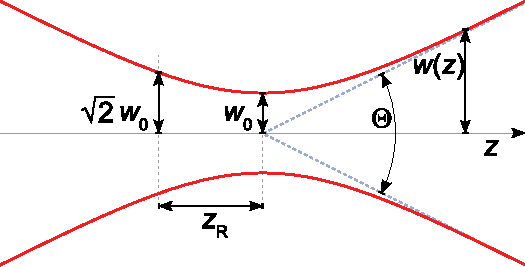
\includegraphics[width=0.4\linewidth]{figures/GaussianBeam.pdf}
	\caption{Gaussian beam profile and some key parameters used in this work, the beam waist $w_0$ and Rayleigh range $z_R$. Figure adapted from \cite{Hermans2009}.}
	\label{fig:GaussianBeam}
\end{figure}


\section{Loading Single Atoms}\label{sec:LoadingAtoms}

For the quantum register, an array of single atoms is needed. In order to do this, individual atoms from the cold atom cloud are loaded in optical tweezers, or tightly focused laser beams. We can write the dynamics of the number of atoms $N$ in the tweezer as \cite{Schlosser2002}

\begin{equation}\label{LoadingTweezer}
	\frac{\text{d}N}{\text{d}t} = \alpha - \gamma N - \beta N(N-1)
\end{equation}

where the first term $\alpha$ is the loading rate or the amount of Rb atoms entering the tweezer per second. Next, $\gamma$ is the atom loss as a result of collisions with the background gas. Lastly, $\gamma$ is a measure for the mainly 2 body loss as a result of light-assisted collisions. No additional laser is required for this, the MOT beams can be used for this purpose.  

We are interested in the case $\beta \gg \gamma$: the two-body collisions are dominant. We can now look at two distinct scenarios:

\begin{itemize}
	\item Starting from 0 atoms in the tweezer: an additional atom entering will now load the tweezer to $N=1$. 
	
	\item Starting from $N=1$: when an additional atom is loaded, the atoms will immediately kick out each other because of the tiny tweezer volume and strong light intensity from the MOT beams. 
\end{itemize}

Apparently, a loading event can lead to either 0 or 1 atom in the tweezer, both with $50\%$ probability. This is known as the collisional blockade effect. Experimentally demonstrated by \cite{Schlosser2001} and \cite{Schlosser2002} showed this effect to exits for 3 orders of magnitude in the loading rate $\alpha$.

Experimentally, $\beta \gg \gamma$ can be keeping $\gamma$ to a minimum by going to the ultra high vacuum regime. We intent to go to a pressure of the order of $10^{-10}$ mbar. In addition $\beta$ is maximized by going to high light-intensities and small trapping volumes. 

\chapter{Generating Tweezer Arrays}\label{ch:arrays}For a quantum computer, multiple qubits are needed that are capable of interacting with each other. Thus, we need to make an array of the tweezers described in \cref{ch:tweezer}, spaced from each other in the order of micrometers. This can be done by sending different laser beams to the objective, all under slightly different angles. Experimentally, this can be realized by an \ac{AOD}: a device that diffracts light off of a sound wave in a crystal, where the degree of diffraction is controlled by a RF signal. By using 2 AODs in an orthogonal configuration, 2D Arrays can be realized \cite{Manuel2016}.

This chapter is on another method of making arrays of tweezers: the spatial light modulator. This device prints a hologram onto a laser beam, such that the interference pattern from this hologram in the focal plane of a lens yields any arbitrary array of spots. Spatial light modulators are thought to enable scaling to higher number of tweezers because when correctly used it can improve uniformity. In principle it is even possible to go make 3D arrays. 

\section{The Spatial Light Modulator}

The \ac{SLM} can manipulate properties of light like amplitude, phase and polarization. The type of SLM used is the phase-only SLM, and as the name suggests it can only control the phase of the light field. It does this by deploying a large array of pixels, where each individual pixel has a liquid crytal in it. The orientation of the crystal will change the refractive index because of the birefringence effect. The pixelated display is manufactured on a layer of silicon to address the voltage of each cell invididually. A sketch of the SLM pixels is shown in \cref{fig:LCoS}.

The working principle of this type of SLM has been documented extensively within our group, for example by \cite{Dijk2012,Bijnen2013,Bijnen2015}. 

\begin{figure}
    \centering
    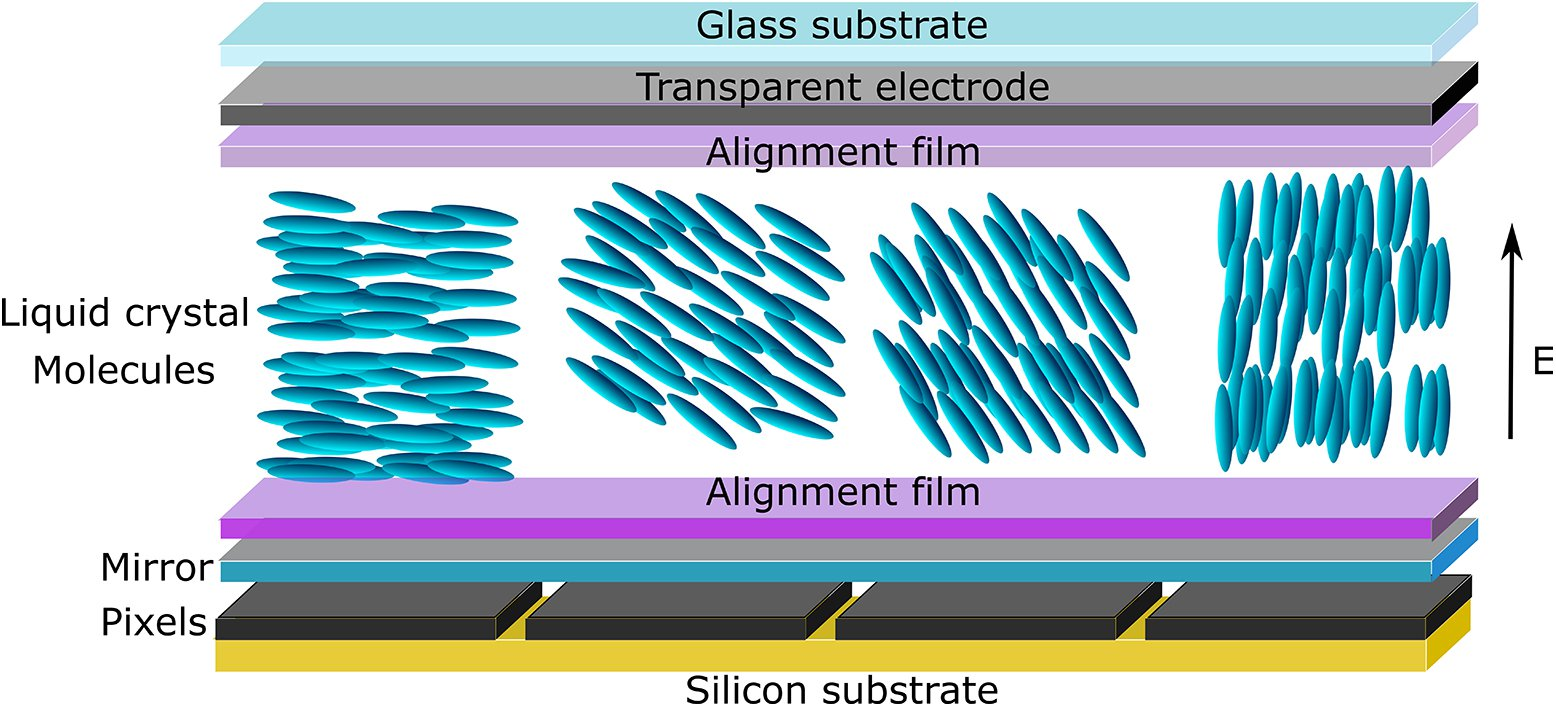
\includegraphics[width=0.6\linewidth]{figures/LCoS.png}
    \caption{The orientation of the liquid crystal cells changes as a function of the applied electric field $E$.}
    \label{fig:LCoS}
\end{figure}

\section{Phase Modulation}

In a phase only \ac{SLM}, each pixel can locally retard the field. As a result of diffraction, one can create arbitrary interference patterns in in the focal plane of the lens as shown by \cite{Bijnen2013}. The birefingence effect means the \ac{SLM} has two different refractive indices, somewhat confusingly called the ordinary and extraordinary refractive indeces respectively ($n_o$ and $n_e$). If the liquid crystal has a thickness $t$, the phase retardation will be $\phi_o = k t n_o$ and $\phi_e(V) = k t n_e(V)$ respectively, such that the phase retarder can be represented by the jones matrix

\begin{equation}\label{eq:JonesMatrix}
    M = e^{i \phi_0} 
    \begin{pmatrix}
        e^{i(\phi_e-\phi_o)} & 0\\
        0 & 1
    \end{pmatrix}
\end{equation}

Thus the phase retardance $\phi$ as a function of the applied voltage is

\begin{equation}
    \phi(V) = \frac{2\pi}{\lambda} (n_e - n_0) t
\end{equation}

This proces can be done separately for each pixel. Typically an SLM has in the order of 2 million pixels. This is shown in \cref{fig:SLMgeometry}





\section{Finding the Hologram}\label{sec:IFTA}

We consider an ensemble consisting of the SLM and a perfect lens with focal length $f$. We define two cartesian coordinate systems: the SLM plane by $\{x',y'\}$ and the focal plane of the lens by $\{x,y\}$. The situation is sketched in \cref{fig:SLMLens}

We adapt the following notation, the \ac{SLM} plane, with individual pixels indexed by $j$, such that the coordinates are $x'_j, y'_j,0$ ($z'=0)$ because by definition the pixels lie in this plane. Next, we place a lens with focal length $f$ one focal length away from the SLM plane. One focal plane further is the focal plane of this Fourier lens, which we call the Fourier plane. See \cref{fig:SLMgeometry}. 

\begin{figure}
    \centering
    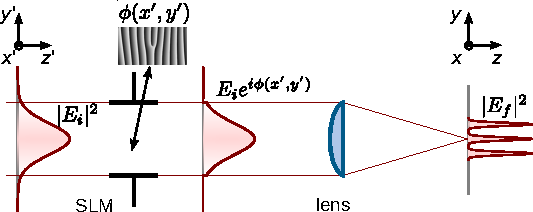
\includegraphics[width = 12cm]{figures/SLMfigure.pdf}
    \caption{Field with intensity distribution $|U_i|^2$ impinging on the SLM, which due to its finite size acts as an aperture. The lens makes the resulting image $|U_f|^2$ in its focal plane. Also shown: two cartesian coordinate systems in the SLM and focal plane. Not to scale. Adapted from \cite{Labuhn2016}.}
    \label{fig:SLMLens}
\end{figure}

When no phase is applied onto the SLM, the lens will focus all the light down to a diffraction-limited in the Fourier plane origin ($x=y=z=0$). As result of traveling from the $j$th pixel to the $m$th trap, under paraxial approximation, the light picks up a phase along the way of 

\begin{equation}
    \Delta_j^m = \frac{2\pi z_m}{\lambdaup f^2}(x_j^2+y_j^2)+\frac{2\pi}{\lambdaup f}(x_j x_m +y_j y_m)
\end{equation}

In the slm plane, we assume uniform illumination of the SLM such that the amplitude is the same $|U_i|$ everywhere. The SLM imprints a phase $\phi(x',y') = \phi_j$, such that the complex amplitude in the SLM plane for pixel $j$ is

\begin{equation}
    U_j(x',y') = |U_j| e^{i \phi_j}
\end{equation}

The contribution for the $m$th trap can be found by summing over all pixels, also keeping track of a phase factor in what is known as the diffraction formula:

\begin{equation}\label{eq:DiffractionFormula}
    \nu_m = e^{i k \left(2 f + z_m\right)}
    \frac{d^2}{i \lambda f} \sum_{j=1}^N e^{i(\phi_j - \Delta_j^m)}
\end{equation}

We assumed uniform illumination of the \ac{SLM}: $|U_j| =1$ everywhere. Furthermore $d$ is the pixel pitch of the SLM. But we are not interested in the phase of each in every spot, but only in the intensity. We will thus emit the prefactors in \cref{eq:DiffractionFormula} and normalize over $N$ pixels

\begin{equation}\label{eq:Vm}
    V_m = \frac{1}{N} \sum_{j=1}^N e^{i(\phi_j - \Delta_j^m)}
\end{equation}

While the algorithm works for 3D spot arrays, in this work we are primarily intersted in 2D arrays. Setting $z=0$ in \cref{eq:Vm} yields 

\begin{equation}
    V_m = \frac{1}{N} \sum_j \exp{\left(i\phi_j\right)} \exp{\left(
    - i 2\pi \left[
    \frac{x_m}{\lambdaup f} x_j + \frac{y_m}{\lambdaup f} y_j
    \right]
    \right)}
\end{equation}

Which is the 2D \ac{DFT} of $e^{i\phi}$ evaluated at spatial frequencies $x_m/\lambdaup f$ and $y_m/\lambdaup f$ in $x$ and $y$ respectively \cite{DiLeonardo2007,Bijnen2015}. The DFT can be efficiently evaluated on a computer using a \ac{FFT}. We stress that the FFT can only be used for 2D arrays. Thus in 2D, we have the following relation:

\begin{equation}
    V_m \propto \text{DFT}\left\{e^{i\phi(x',y'} \right\} 
    \left(x_m / \lambdaup f,y_m / \lambdaup f\right)
\end{equation}                                






\begin{equation}
    \centering
    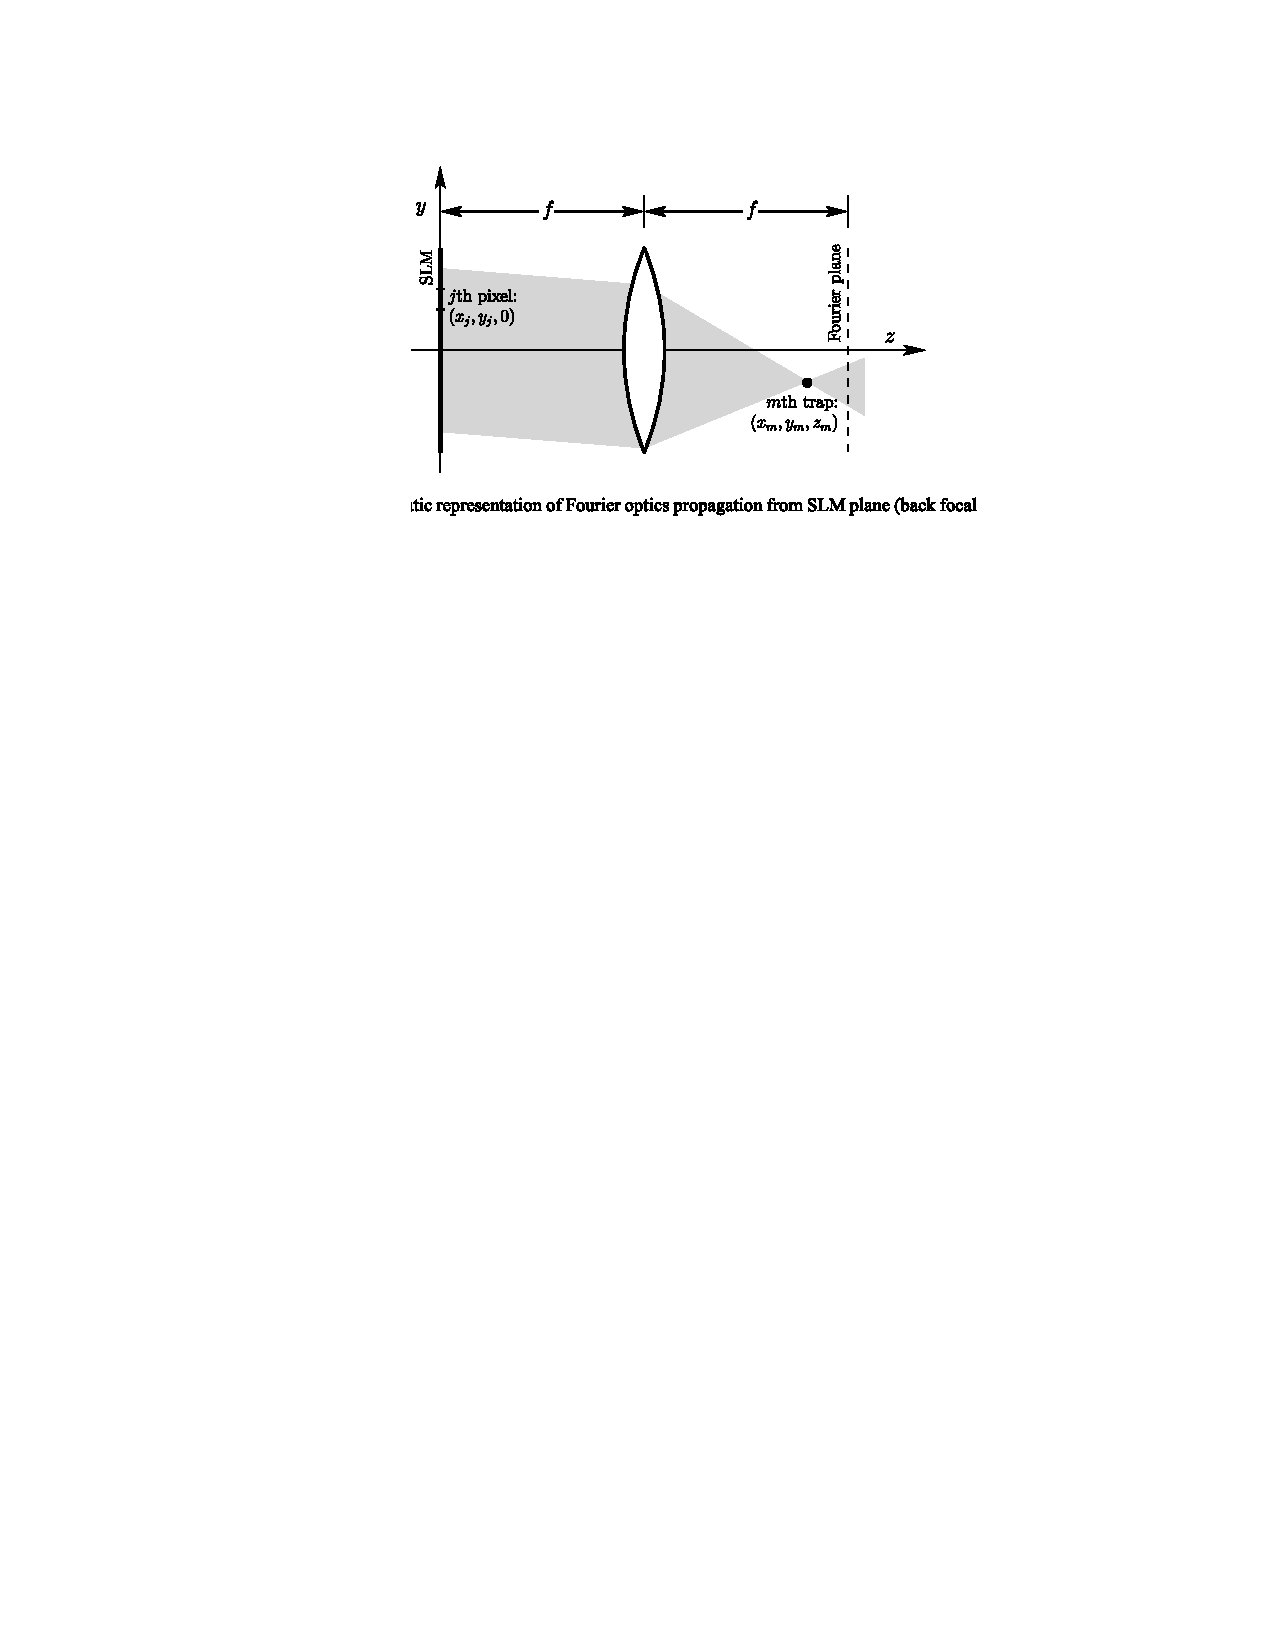
\includegraphics[width=0.\linewidth]{figures/SLMgeometry.pdf}
    %\caption{SLM and Fourier plane, each with their own coordinate labeling.}
    \label{fig:SLMgeometry}
\end{equation}





$U_f$ and $U_i$ are known in an experiment. Thus if one finds the right phase pattern or hologram $\phi(x,y)$, any intensity distrubution can be found from \cref{FourierLens}. But a single inverse inverse fast Fourier transform (IFFT) will not suffice, because this will not modulate the phase contributions of the invididual pixels $\phi_{kl}$ but also the amplitude contributions, which a phase-only SLM, by far the most commonly used SLM, cannot do. 

Instead, a set of algorithms known as inverse Fourier transform algorithms (IFTA) were pioneered by \cite{Hirsch1971} and adapted by \cite{Gerschberg1972} to tackle this task. The goal of the algorithm is to find a phase pattern for the SLM, such that in the focal plane of the lens, the light intensity $I_m = |V_m|^2$ in invidual spots $m$ is optimized in terms of parameters diffraction efficiency efficiency $e$ and uniformity of the spots $u$ \cite{DiLeonardo2007}:

\begin{equation}\label{EfficiencyUniformity}
    e = \sum_m |V_m|^2, \quad u= 1-\frac{\text{max}(|V_m|^2)-\text{min}(|V_m|^2)}{\text{max}(|V_m|^2)+\text{min}(|V_m|^2)}
\end{equation}

These are theorical quantities and not actually measured. The algorithm works essentially by virtually propagating light back and forward in iterations acoording by computing FFT and IFFT's, applying constraints in the focal and SLM plane in each iteration. 




In order to overcome this issue, after the inverse FFT we replace the computed complex amplitude by our incident amplitude $PU_0$ and we compute its FFT, returning again to the focal plane. Here, we replace the obtained obtained complex amplitude for the desired amplitude $|U(x,y)|^2$. This process is iterated several times until convergence is reached. This family of algorithms is refered to as an inverse Fourier transform algorithm (IFTA) and essentially consists of virtually propagating light back and forward between the input and focal planes. 

IFTA algorithms were pioneered in\cite{Hirsch1971} and adapted for phase retrieval by \cite{Gerschberg1972}. The implementation of the IFTA algorithm was done by \cite{Bijnen2013,Bijnen2015}. It was adapted to achieve better convergence by defining a signal window, within it the desired pattern is made. Outside of this window, the amplitude is unconstrained. This relaxiation of constraints allows for better convergence of the desired pattern, at the cost of energy lost outside of the window \cite{Bijnen2013,Bijnen2015}.

\section{Operating the SLM}

The algorithm as explained in \cref{IFTA} was implented in software by \cite{Bijnen2015}. The input intensity $|PU_0|^2$ is assumed to be a plane wave. Using the SLM is explained here. The SLM will inevitably lose power due to several processes. These are explained here. 

\subsection{Diffraction}

Diffraction. The SLM is a device consisting of individual pixels. Therefore, it is essentially a 2D diffraction grating, and light will diffract in several directions. In 1D, we know that according to diffraction theory the diffraction angle maxima $\theta_m$ from a plane wave incident at $\theta_i$ occur at $\theta_m = \arcsin(\sin\theta_i - m\lambdaup/d)$, where $m$ is the order of diffraction and $d$ the pixel pitch. We are interested in the light in the $m=0$ diffracton order, other orders are spatially filtered out and unused.

\subsection{Zeroth Order}

Light can reflect on the spacings between the pixels. Also, it can reflect off of the electrodes at the back of the device. All of this undiffracted light is focussed onto the optical axis by the objective. As a result, the optical axis unusable to shape light and we have to seperate our modulated light from this 'zeroth order peak'. This is done by superimposing a linear phase on top of the SLM phase pattern. Because the phase is computed modulo 2$\pi$ the resulting pattern is a blazed grating. Light from the higher diffraction orders and zeroth order peak can be blocked by an iris in the focal plane of an intermediaty lens. 
    
\subsection{Finite aperture size}

In order to employ the maximum amount of pixels the SLM has to offer, and therefore the maximum drawing area in the focal plane of the Fourier lens, all of the pixels should be illuminated. However, because the incident beam is described by a gaussian, this will lead to power loss as a result of light not falling on the active pixel area. 
    
We can estimate this power loss by shining a Gaussian beam $G(x,y)$ of width $w(z)$ and power $P_0$ onto a rectangular aperture of dimensions $(2S_x, 2S_y)$ where $S_{x,y}$ are the semi-widths of the aperture. The relative power transmission $P/P_0$ can be found by integrating the intensity of the beam \cref{GaussianBeamIntensity} in cartesian coordinates over the aperture

\begin{equation}\label{RectAperturePower}
    \frac{P}{P_0} =
    \iint I(x,y) dA=
    \text{Erf}\left(\frac{\sqrt{2}S_x}{w(z)}\right) \text{Erf}\left(\frac{\sqrt{2}S_y}{w(z)}\right)
\end{equation}

where Erf($\cdot$) denotes the error function. The optimum incident beam size $w(z)$ is thus a compromize between drawing area and power efficiency. We chose $w(z) \approx S_{x}$, specifically $w(z) = 4.8$ mm and $S_x = 4.9$ mm. 

\subsection{Reflectivity}

As can be seen in \cref{fig:LCoS}, the light will back reflect at after passing through the liquid crystal. This back plate will have a non-perfect anti relection coating, leading to some light being absorbed. 


\section{Calibration}

We know that the phase pattern of the SLM is realized by the birefringence effect. However, it turns out the phase retardation as a function of the applied voltage is non-linear. Additionally, the surface of the SLM is not fully flat, introducing a small aberration. Both of these effects differ for indiviual SLM units, even for the same model. Therefore, here we will briefly review how to calibrate the SLM to account for these two effect.s 

\subsection{Electro-Optic Response}

The goal of the calibration of the phase as a function of applied voltage (electro-optic response) is to 

\begin{enumerate}
    \item Achieve a linear electric-optic response. 
    \item Ensure the phase is modulate by a full wave $2\pi$ spanning the minimum to the maximum grey level. 
\end{enumerate}

\subsection{Optical flatness correction}

Because of the silicon producetion process, the chip is not completely flat. The optical flatness of SLM was measured to be $0.18\lambdaup$ by manufacturer Meadowlark. Additionally, the manufacturer measured the shape of the correction using Michelson interferometry. By substracting this measured non-flatness from the calculated phase pattern, this effect can be corrected. 


\section{Arrays of tweezers}

\subsection{Array Spacing}

Because of the properties of the Fourier transform, the smallest possible 

\subsection{Spot Detection}

We make an arbitrarily sized array of optical tweezers. For detecting maxima locations, we could simply set pixels above a certain count threshold as a maxima. The disadvantage of this is that a noisy pixel could be detected as a spot, which would hinder analysis. 

To combat this, we first convolute the image with a Laplacian of Gaussian filter, which first smoothes the image to reduce noise. Subsequently it computes the 2D laplacian to detect edges. If this second derivative is above a certain threshold, we detect the edge as a spot. If the detected amount of spots is not the expected amount, we can easily tune the threshold. The camera image is cropped into regions of interest around the spots marked by the Laplacian of Gaussian filter. 

\subsection{Spot Fitting}

Our tweezers should be described by \cref{FourierBesselAperture}. However, because of a lack of an analytic expression this is not the most convenient. \cref{FourierBesselAperture} can closely be resembled by a Gaussian. We will therefore use the following function for fitting spots numbered $k$

\begin{equation}\label{2DGaussian}
    G_k(x,y) = U_k \exp{\left(-\frac{(x_k-x_{k,0})^2}{2\sigma_{k,x}^2}\right)}
    \exp{\left( \frac{-(y_k-y_{k,0})^2}{2\sigma_{k,y}^2} \right)}
\end{equation}

Here $U$ is the 'trap depth', $x,y$ are the cartesian coordinates in the camera frame and $x_0,y_0$ is the center of the spot. Lastly $\sigma_{x,y}$ are standard deviations in $x$ and $y$. In principle, because the limiting aperture in the system is a circular aperture, the spots should be more or less symmetric and $\sigma_x\approx \sigma_y$ which we confirmed. We find the $1/e^2$ waist $w_k=\sigma_{k,x}+\sigma_{k,y}$. 
\chapter{Implementation in the Machine}\label{ch:implementation}%\section{Rb Magneto Optical Trap}

Our journey starts with a cloud of ultracold atoms, because the tweezers are not deep enough to load room temperature atoms. Also, we need ultracold temperatures to avoid decoherence. The gas cloud is prepared using a 3D magneto optical trap (MOT). The MOT consists of 3 circularly polarized laser slightly detuned from the 780 nm D2 line of Rb-87, as well as a repump laser. The magnetic field gradient is provided by a set of coils in the standard anti-Helmholtz configuration. 

\subsection{Atom Source}

For our atom source we use a rubium dispenser. Atoms are released when the power supply is turned on. 

Here, a detailed overview will be given of the setup built for the optical tweezers experiment. The overview is split in three parts, each with their own section. 

\section{Glass Cell}

Light from a 780 Toptica laser diode is coupled in and out of a Thorlabs FC780 fiber. As it comes out of the fiber, it is sent through a polarizing beam splitter cube. To ensure maximum power transmission through the cube, the polarization of the light is rotated using a half wave plate. 

The fiber outcoupler yields a beam waist of 1.05 mm. The light is matched to the dimensions of the SLM using a Keplarian telescope consisting of a set of lenses with focal lengths $f_1=150$ mm and $f_2=500$ mm. This yields a beam waist of 1.05 mm $(f_2/f_1) \approx 3.5$ mm.

The SLM has dimensions $8$ by $15$ mm. Because this is larger than the beam waist, the power loss as a result of its aperture is limited. test

\section{Imaging Tweezer Arrays}

\section{Detecting Atoms}

The beamsize from the SLM is sent to a high numerical aperture (NA) infinity-corrected microscope objective. Additionally, it has a long working distance of 15.08 mm because it is aberration-corrected for use with a 3.5 mm cover glass. We chose the Mitutoyo G Plan Apo 50X. It's specifications are shown in \cref{table:MitutoyoSpecs}.      

\begin{table}[h]
    \caption{Mitutoyo specifications.}
    \label{table:MitutoyoSpecs}
    \centering
    \begin{tabular}{l | l}
        \textbf{Metric}                  & \textbf{Specification} \\ \hline
        NA                               & 0.5                    \\ \hline
        working distance                 & 15.08 mm               \\ \hline
        Equivalent focal length          & 4 mm                   \\ \hline
        Compatible cover glass thickness & 3.5 mm                
    \end{tabular}
\end{table}

From this we can deduct a back pupil radius $d/2 = 2 f_{\text{eff}} \text{NA} = 2$ mm. where $f_\text{{eff}}$ is the equivalent focal length. The beam from the SLM is steered to the Mitutoyo while meanwhile passing a lens relay system, mapping the SLM plane onto the back input plane of the high NA objective. 

\subsection{Relay Lenses}

The relay system serves several functions

\begin{enumerate}
    \item Avoid clipping. The SLM prints an angular phase pattern. When the distance between SLM and the objective becomes too large, the beam will clip on the pupil. The telescope is designed such that the planes at SLM and the Mitutoyo are conjugated, meaning that for any field the output is centered on the Mitutoyo. 
     
    \item Decrease beam waist. If the 3.5 mm waist from the SLM is directed to the Mitutoyo, we would lose a significant amount of power. The transmission $P/P_0 = 1- \exp{(w_i^2/R^2)} \approx 87.5\%$ for $w_i/R = 1$. Where $w_i$ is the input beam waist and $R$ the pupil radius. Therefore, the beam size is decreased by a second telescope to $w_i \approx 2$ mm.
    
    \item In an intermediate focus point in the telescope, the spot image is produced. This allows filering out unwanted diffraction orders and undiffracted light. 
\end{enumerate}

To ensure no clipping \cite{Nogrette2014}, the lenses should be placed in a 4f configuration. Additionally, the distance from the second relay to the objective should accomodate sufficient distance for the optics needed to fit in between: a polarizing beam splitter to recombine the moving beam from the acousto-optical deflectors, a dicroic mirror to split off fluoresence and a mirror to steer the beam into the vertical direction. A CAD drawing puts a conservative estimate of $f_2 \approx 400$ mm here.

Concerning the second point, the magnification $m$ should be 

\begin{equation}\label{magnification}
    m = \frac{f_2}{f_1}= \frac{R}{w(z)} \approx 0.42
\end{equation}

where $f_2$ and $f_1$ are the focal lengths of the second an first relay lenses, $R = 2$ mm is the aperture radius of the objective and $w(z) = 4.7$ mm is the beam waist from the fiber collimator. \cref{magnification} puts the total length of a full 4f relay telescope at $2f_1+2f_2 \approx 2.7$ m. 

To shorten this beam size, our partner group at University of Amsterdam make use of the versatility of the SLM to program the first relay lens in the SLM itself. However, to still satisfy all of the requirements some of the lens spacings will have to be adapted. This can be understood in terms of the ABCD matrix formalism. Consider the matrix $M$ describing a telescope with spacings according to the 4f configuration: 

\begin{equation}\label{ABCD_telescope}
    M_{4\text{f}} = 
    \begin{bmatrix}
        1 & f_2\\
        0 & 1
    \end{bmatrix}
    \begin{bmatrix}
        1 & 0\\
        -1/f_2 & 1
    \end{bmatrix}
    \begin{bmatrix}
        1 & f_1+f_2\\
        0 & 1
    \end{bmatrix}
    \begin{bmatrix}
        1 & 0 \\
        -1/f_1 & 1
    \end{bmatrix}
    \begin{bmatrix}
        1 & f_1 \\
        0 & 1
    \end{bmatrix} 
\end{equation}

Now, consider the situation where the SLM acts directly as the first lens with focal length $f_1$. Then it can be shown we have the following matrix:

\begin{equation}\label{LensSLM}
    M_{\text{SLM}} = 
    \begin{bmatrix}
        1 & L_{23}\\
        0 & 1
    \end{bmatrix}
    \begin{bmatrix}
        1 & 0\\
        -1/f_2& 1
    \end{bmatrix}
    \begin{bmatrix}
        1 & L_{12} \\
        0 & 1
    \end{bmatrix}
    \begin{bmatrix}
        1 & 0\\
        -1/f_1& 1\\
    \end{bmatrix}
\end{equation}

Solving $M_{\text{4f}} = M_{\text{SLM}}$ yields: a focal length for the second lens of $f_2 = 285$ mm, which is hard to find. However, we can enforce $f_2 = 300$ mm, relaxing requirement 1. and this will only slightly change the other parameters. Final result: $f_1 = 714$ mm, $L_{12} = 1014$ mm and $L_{23} = 426$ mm. 

\section{Rb System}

The laser system and optical frequency reference for Sr is set to arrive after this thesis was written. Additionally the atom source consisting of an oven, Zeeman slower and deflection stage was only in the design stage at the time of writing (\cref{fig:SrLoading}). Therefore, we resorted to using rubidium as an ultra cold atom source first. This allows us to test our arrays of optical tweezers. The only adjustment that needs to be done for this is the wavelength, which as it turns out happens to be minor and well within the tuning range of our titanium sapphire crystal. 

\subsection{Vacuum System and Atom Source}

The rubidium vacuum system was built by Deon Janse van Rensburg and Rik van Herk. It consists of an optically contacted glass cell (out diameter 30 mm, glass thickness 4 mm) kindly supplied by collaborators from UvA. As atom source, a triplet of Rubidium dispensers are used, powered by a power supply typically running at 5 ampères. As for pumps, a turbo pump was used for initial pumpdown to $p\sim 10^{-8}$ mbar after which an combination sputter ion pump and a non evaporative getter\footnote{NEXTorr Z 100} take over. We reached a some $p \sim 2 \cdot 10^{-10}$ mbar, after baking the system at 130${}^{\circ}$C for two weeks. This is described in the thesis of Rik van Herk \cite{Herk2022}.

\subsection{Laser System}

The atomic species that we selected to cool is \textsuperscript{85}Rb because it is the most abundant. A \textsuperscript{85}Rb requires a cooling laser detuned from the D-2 line of Rb, as well as a repump laser to cycle back atoms in the cooling transition that end up in the wrong ground state. The laser system was already in the lab, built primarily by \cite{Reijnders2010}. It used a separate repump laser (Toptica DL100, $P \sim 100$mW) from the trapping/cooling laser (Toptica DLX100, $P \sim 500$mW). 

After numerous components from the repump laser system broke, we decided to omit the seperate repump laser and put sidebands on the trapping laser using an electro optic modulator (EOM) instead, as the small amount of power lost in the trapping laser is not of critical importance for us. The laser system is sketched in \cref{fig:RbLaserSetup}. The fiber on the lower left is where previously both the trapping and repump laser would be fiber coupled for a frequency offset lock system, which we replaced by a (fiber coupled) wavemeter. 

The system consists of a laser detuned by an acousto-optic modulator. For long term stability, the laser is frequency locked using a modulation transfer spectroscopy setup \cite{McCarron2008,Reijnders2010}. In order for the laser to be in resonance with the Rb spectroscpopy cell, an AOM is used with the same frequency as the AOM going to the MOT. 

\subsection{Repump Sidebands}

In order to make the sidebands, an EOM was used. An EOM uses phase modulation to create sidebands with shifted frequencies. The amount of sidebands is determines by the modulation depth. The power in the various sidebands as a function of the modulation index $\epsilon$ is described by \cite{McCarron2008}

\begin{equation}
    E = E_0 \left[
        \sum_{n=0}^{\infty} J_n(\eta)\sin{(\omega_c+n\omega_n)t}+
        \sum_{n=1}^{\infty} (-1)^n J_n(\eta) \sin{(\omega_c-n\omega_m)t}
    \right]
\end{equation}

where $t$ is time and $\omega_c$ the carrier frequency. If $\epsilon <1$ most of the power is contained in the zeroth order (unmodulated) beam and a small fraction is contained in the first sidebands. The sidebands are always symmetric from the zeroth order, but we only use one of them, the other is wasted. 

The EOM\footnote{7Qubig EO-Rb85-3K} was fed a $f = 2915$ MHz signal provided by a harmonic synthesizer RF \footnote{DS instruments SG6000PRO} providing a signal of $-6.9$dbm. This signal was amplified by a 45 dB amplifier \footnote{Minicircuits ZHL-16W-43+} which should provide some $\sim 15$\% of power in the first sidebands \cite{Rens2014}, which should be a sufficient amount of power for a repump laser. 

\begin{figure}
    \centering
    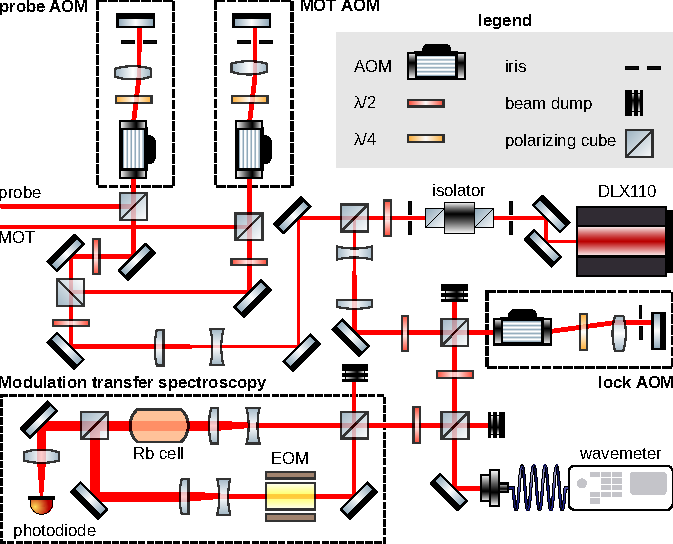
\includegraphics[width=\linewidth]{figures/RbLaserSetup.pdf}
    \caption{Laser system for the trapping and repump laser system for \textsuperscript{85}Rb. The bulk was already built by \cite{Reijnders2010}. All beam splitter cubes shown are polarizing. The Rb vapor cell is heated to 150${^{\circ}}$C.}
    \label{fig:RbLaserSetup}
\end{figure}


\chapter{Conclusions and Outlook}\label{ch:conclusion}%conclusies


\clearpage
\chapter*{Bibliography}
\addcontentsline{toc}{chapter}{Bibliography}%in inhoud

\printbibliography[heading=none]



\begin{appendices}

 %appendix nummering sections, equations, figures5
\renewcommand{\thesection}{\thechapter.\arabic{section}}
\renewcommand\thefigure{\thechapter.\arabic{figure}}
\renewcommand\theequation{\thechapter.\arabic{equation}}
 
 \setcounter{equation}{0}
 \setcounter{figure}{0}
 
 \chapter{Pauli Strings}\label{ch:PauliExpectation}

In VQE, the Hamiltonian is decomposed in Pauli strings $P_{\alpha}$.

\begin{equation}
	\mathcal{H} = \sum_{\alpha} h_{\alpha} P_{\alpha}
\end{equation}


A Pauli string is a tensor product of Pauli matrices $\sigma_j^{\alpha} \in \{\mathcal{I}, \sigma_j^x, \sigma_j^y, \sigma_j^z\}$ where $\mathcal{I}$ is the identity matrix and $\sigma_j^{\alpha}$ are the standard Pauli spin matrices \cite{Griffiths2004}

\begin{equation}
	\mathcal{I} =
	 \begin{pmatrix}
		1 & 0\\
		0 & 1
	\end{pmatrix},
	 \quad \sigma_j^x=
	\begin{pmatrix}
		0 & 1\\
		1 & 0
	\end{pmatrix},
	\quad \sigma_j^y=
	\begin{pmatrix}
		0 & -i\\
		i & 0
	\end{pmatrix} 
	\quad \text{and}
	\quad \sigma_j^z = 
	\begin{pmatrix}
		1 & 0\\
		0 & -1
	\end{pmatrix}
\end{equation}

Such that the Pauli string is \cite{Moll2018}:

\begin{equation}\label{eq:PauliString}
	P_{\alpha} = 
	\sigma_1^{\alpha_1} \otimes \sigma_2^{\alpha_2} \otimes \ldots \otimes \sigma_N^{\alpha_N} = 
	\bigotimes_{j=1}^N \sigma_j^{\alpha_j}
\end{equation}

This has the nice property that estimating the Hamiltonian is equivalent to measuring populations of individual qubits. This has to be done repeatedly, to get an estimate. Using the definition for the expectation value for $\sigma_j^z$ for example yields

\begin{equation}\label{eq:ExpectationValue}
	\bra{\psi}  \sigma_j^z  \ket{\psi} = 
	\begin{pmatrix}
		a & b
	\end{pmatrix}^{\dag}
	\begin{pmatrix}
		1 & 0\\
		0 & -1
	\end{pmatrix}
	\begin{pmatrix}
		a \\ b
	\end{pmatrix}=
	|a|^2-|b|^2
\end{equation}

Expectation values of tensor products of Pauli strings can be found similarly \cite{LaRose2021}. For a string of 2 Pauli matrices, for example, $\sigma_j^x$ and $\sigma_j^y$, use need the two-qubit definition \cref{eq:TwoQubits} to find

\begin{equation}\label{eq:ExpectTensor}
	\bra{\psi_{2q}}( \sigma_j^x \otimes \sigma_j^ y) \ket{\psi_{2q}} 
	= |\alpha_{00}|^2 - |\alpha_{01}|^2 - |\alpha_{10}|^2 + |\alpha_{11}|^2.
\end{equation}








 \chapter{Light-Matter Interaction}\label{ch:LightMatter}

We follow \cite{Leeuwen2017}. For a 2-level atom (see \cref{fig:2LevelAtom}), the atomic Hamiltonian is best written down in its eigenstates, such that we have 

\begin{equation}\label{eq:AtomHamiltonian}
	\mathcal{H}_A = \hbar \omega_g \ket{g}\bra{g} + \hbar \omega_e \ket{e}\bra{e}
\end{equation}

Where the eigenvalues are $\hbar \omega_g$ and $\hbar \omega_e$, and they satisfy the Schrodinger equation

\begin{subequations}\label{eq:AtomEigenStates}
	\begin{align}
		i \hbar \dot{\ket{g}}= \hbar \omega_g \ket{g}, \\
		i \hbar \dot{\ket{e}}= \hbar \omega_e \ket{e}
	\end{align}
\end{subequations}

Where the dote denotes the temporal derivative. We treat the light field as a time-dependent perturbation $H_{I}(t)$ such that the total Hamiltonian is

\begin{equation}\label{eq:Perturbation}
	\mathcal{H} = \mathcal{H}_A + \mathcal{H}_{I}(t),
\end{equation}

The time evolution of \cref{eq:Perturbation} can be written down in the unperturbed states as

\begin{equation}\label{eq:TwoLevel}
	\ket{\psi} = c_g(t) e^{-i \omega_g t} \ket{g} + c_e(t) e^{-i \omega_e t} \ket{e}.
\end{equation}

Substituting \cref{eq:Perturbation,eq:TwoLevel} in the Schrodinger equation yields, after canceling the terms that involve \cref{eq:AtomEigenStates} 

\begin{equation}\label{eq:TwoLevelSchroedinger}
	i \hbar \left(\dot{c}_g(t) e^{-i \omega_e t}+\dot{c}_e(t) e^{-i \omega_e t} \right) = c_g(t) \mathcal{H_I}(t)\ket{g} e^{-i \omega_g t} + c_e(t) \mathcal{H_I}(t) \ket{e} e^{-i \omega_e t},
\end{equation}

Because $\{\ket{g},\ket{e}\}$ constitute an orthogonal set, we can exploit a trick where we multiply \cref{eq:TwoLevelSchroedinger} from the left by $\{\bra{g},\bra{e}\}$, yielding a set of two coupled equations:

\begin{subequations}\label{eq:CoupledEq}
	\begin{align}
		i \hbar \dot{c}_g &= e^{-i \omega_0 t} 
		\left[c_g \bra{g} \mathcal{H}_I \ket{g} + c_e \bra{g} \mathcal{H}_I \ket{e}\right]  \\
		i \hbar \dot{c}_e &=  e^{ i \omega_0 t} 
		\left[c_g \bra{e} \mathcal{H}_I \ket{g} + c_e \bra{e} \mathcal{H}_I \ket{e}\right] .
	\end{align}
\end{subequations}

Where the explicit time dependence of $c_g$ and $c_e$ will be omitted from now on. In order to calculate the matrix elements in \cref{eq:CoupledEq}, the Wigner-Eckart theorem can be used. If $\ket{g}$ and $\ket{e}$ are described by the quantum numbers $J$, $M$ and $\alpha$ (total and magnetic quantum number, and $\alpha$ keeps track of the other quantum numbers), the matrix elements can be evaluated as 

\begin{equation}\label{eq:WignerEckart}
	\bra{J_g M_g \alpha_g} \hat{T}_q^n \ket{J_e M_e \alpha_e} = 
	(-1)^{J_e-M_e} \begin{pmatrix}
		J_e & n & J_g \\
		-M_e& q & M_1
	\end{pmatrix}
	\bra{J_g\alpha_e } | \hat{T}^n | \ket{J_g\alpha_g }
\end{equation}

Where $q \in \{-1,0,1\}$ is the spherical component index, the 2 x 3 matrix is the $3j$-symbol, which is in principle known and can be formulated in terms of  Glebsch-Gordan coefficients. $\hat{T}_q^n$ is a spherical tensor operator. The term $\bra{}|\hat{T}^n|\ket{}$ is the reduced matrix element \cite{Leeuwen2017}. Calculating the matrix elements will not be done here, but many $3j$-symbols will turn out to be zero. For example, the diagonal matrix elements will turn out to be zero, such that \cref{eq:CoupledEq} reduces to

\begin{subequations}\label{eq:NoOffDiagonal}
	\begin{align}
		i \hbar \dot{c}_g &= e^{-i \omega_0 t}  c_e \bra{g} \mathcal{H}_I \ket{e} \\
		i \hbar \dot{c}_e &=  e^{ i \omega_0 t} c_g \bra{e} \mathcal{H}_I \ket{g}  .
	\end{align}
\end{subequations}


We will now calculate the matrix elements for the classical light field. Up until this point, the derivation was exact for the 2-level atom. Now we will make a series of approximations to get to a solvable set of equations \cite{Leeuwen2017}

\begin{equation}\label{eq:CosineLightField}
	\mathbf{E}(z,t) = \mathbf{E}_0 \cos{(k z - \omega t)}
\end{equation}

Under the dipole approximation, the interaction Hamiltonian is \cite{Foot2005}

\begin{equation}
	\mathcal{H_I} = - e\mathbf{r}\cdot \mathbf{E}
\end{equation}

Because an atom is orders of magnitude smaller than the wavelength of the radiation field, we can safely set $z=0$. The Hamiltonian simplifies to 

\begin{equation}\label{eq:OscillatingHamiltonian}
	\mathcal{H}_I = \frac{-e E_0 z}{2} \left(e^{i \omega t} + e^{-i \omega t}\right)
\end{equation}

Substitution of \cref{eq:OscillatingHamiltonian} in \cref{eq:NoOffDiagonal} yields

\begin{subequations}\label{eq:ClassicalHamSubstituted}
	\begin{align}
		i \hbar \dot{c}_g &= \frac{e E_0}{2} c_e[e^{ i (\omega-\omega_0) t}+e^{-i(\omega+ \omega_0)t}] \bra{g} z \ket{e} \\
		i \hbar \dot{c}_e &= \frac{e E_0}{2} c_g[e^{+i (\omega+\omega_0) t}+e^{-i(\omega- \omega_0)t}] \bra{e} z \ket{g}  .
	\end{align}
\end{subequations}

We assume $\omega \gg \delta$, such that $\omega+\omega_0 \approx 2\omega_0$ which oscillates much faster than the $\omega-\omega_0=\delta$ term. Over time scales of absorption and emission processes, this much faster contribution averages out. This is known as the \ac{RWA} \cite{Vredenbregt2020,Loudon2000} Thus we are left with

\begin{subequations}\label{eq:Rabi}
	\begin{align}
		i \hbar \dot{c}_g &= c_e \frac{\hbar \Omega  }{2} e^{ i \delta t},\\
		i \hbar \dot{c}_e &= c_g \frac{\hbar \Omega^*}{2} e^{-i \delta t}.
	\end{align}
\end{subequations}

Where the so-called Rabi frequency 

\begin{equation}\label{eq:RabiFrequency}
	\Omega \equiv \frac{e E_0}{\hbar} \bra{g}\mathbf{r}\ket{e}
\end{equation}

and its complex conjugate is introduced. In order to remove the time-dependence of \cref{eq:Rabi}, we can turn 'look' at them from a 'rotating frame'. More formally, it is a basis transformation described by the unitary matrix $\mathcal{U}$ \cite{Foot2005}

\begin{equation}\label{eq:RotatingFrame}
	\begin{pmatrix}
		\tilde{c}_g \\ 
		\tilde{c}_e
	\end{pmatrix} =
	\mathcal{U}
	\begin{pmatrix}
		c_g \\
		c_e
	\end{pmatrix} =
	\begin{pmatrix}
		e^{i \delta t/2} & 0\\
		0 & e^{-i \delta t/2}
	\end{pmatrix}
	\begin{pmatrix}
		c_g \\
		c_e
	\end{pmatrix} =
	\begin{pmatrix}
		c_g e^{i\delta t/2}\\
		c_e e^{-i \delta t/2}
	\end{pmatrix}
\end{equation}.

Substituting \cref{eq:RotatingFrame} in \cref{eq:Rabi} yields, after omitting the tiles, the matrix equation \cref{eq:MatrixEvolution}

\begin{equation}
	i \hbar \begin{pmatrix}
		\dot{c}_g \\ 
		\dot{c}e
	\end{pmatrix}
	= \frac{\hbar}{2} \begin{pmatrix}
		\delta & \Omega \\ \Omega^* & -\delta 
	\end{pmatrix} 
	\begin{pmatrix}
		c_g \\ c_e
	\end{pmatrix}.
\end{equation}



%\chapter{Fourier Optics}



% %\section{Fourier Optics}

% For describing the optics in this project, we need a description of diffraction. Ray optics will not suffice for this, wave optics is needed. One elegant description is Fourier optics. 

% We start with a result from Maxwell's equations in an electromagnetic medium in three dimensions, where $\mathbf{u(\mathbf{r},t)}$ can denote either the electric or magnetic field vector.

% \begin{equation}\label{WaveEquation}
% 	\nabla^2 \mathbf{u}(\mathbf{r},t) = \frac{n^2}{c^2} \frac{\partial^2 \mathbf{u}(\mathbf{r},t)}{\partial t^2}
% \end{equation}

% For monochromatic light, which is true to good approximation for a laser, we can substitute the ansatz $\mathbf{u(\mathbf{r},t)} = Re\{ \mathbf{U}(\mathbf{r}) e^{i \omega t} \}$, yielding the time-independent so called Helmholtz equation:

% \begin{equation}\label{Helmholtz}
% 	(\nabla^2 + k^2)  \mathbf{U}(\mathbf{r}) = 0
% \end{equation}

% \section{Huygens-Fresnel Principle}

% The Huygens-Fresnel principle can be expressed mathematically as \cite{Goodman2005}:

% \begin{equation}\label{eq:HuygensFresnel}
% 	U(P_0) = \frac{1}{i \lambda} \iint U(P_1) \frac{e^{i k r}}{r} \cos{\theta} \text{d}x' \text{d}y'
% \end{equation}

% Because $\cos{\theta} = z/r$, we can write \ref{eq:HuygensFresnel} as:

% \begin{equation}\label{eq:HuygensFresnel2}
% 	U(x,y) = \frac{z}{i \lambda} \iint U(x',y') \frac{e^{i k r}}{r^2} \text{d}x' \text{d}y',
% \end{equation}

% where $r$ is given by $\sqrt{(z^2 + (x-x')^2 +(y-y')^2)}$. Because the square root is difficult to work with, $r$ can be approximated by assuming $z^2 \gg (x-x')^2 + (y-y')^2$, which is really the same thing as assuming the angle $\theta$ is small (paraxial approximation). We can then expand the definition for $r$ to first order as

% \begin{equation}\label{eq:FirstOrderR}
% 	r = z \sqrt{1+ \Big(\frac{x-x'}{z}\Big)^2 + \Big( \frac{y-y'}{z}\Big)} \approx z \left[ 1 + \frac{1}{2} \Big(\frac{x-x'}{z}\Big)^2 + \frac{1}{2} \Big( \frac{y-y'}{z} \Big)^2\right]
% \end{equation}

% When $r$ appears in the denominator, we can approximate the term in square brackets as unity. For terms appearing in the exponent however, we cannot do this. Substituting \cref{eq:FirstOrderR} in \cref{eq:HuygensFresnel2}:

% \begin{equation}\label{eq:HuygensFresnel3}
% 	U(x,y) = \frac{e^{i k z}}{i \lambda z}\iint U(x',y') \exp{\frac{i k}{2 z} \left[(x-x')^2+(y-y')^2\right]} \text{d}x' \text{d}y'
% \end{equation}

% \subsection{Fraunhofer Approximation}

% the term in square brackets in \cref{eq:HuygensFresnel3}, when expanded yields:

% \begin{equation}
% 	(x^2+y^2) + (x'x+y'y)+(x'^2+y'^2)
% \end{equation}

% As a final approximation, if the Fraunhofer approximation is met: $2z \gg k \max{(x'^2+y'^2)}$, $x'x+y'y \gg x'^2+y'^2$ and we can drop the latter two terms in the integration. If the constant phase term involving $x^2+y^2$ is brought in front of the integral we are left with the Fraunhofer diffraction integral:

% \begin{equation}\label{FraunhoferDiffractionIntegral}
% 	U(x,y) = \frac{e^{i k z}}{i \lambda z} e^{i(x^2+y^2)/(2z)} \iint U(x',y') e^{\frac{-i 2 \pi}{\lambda z} (x'x+y'y)}\text{d}x' \text{d}y'
% \end{equation}

% In \cref{FraunhoferDiffractionIntegral}, the 2D Fourier transform property can be recognized, for frequencies $f_x=x/(\lambda z)$ and $f_y=y/(\lambda z)$:

% \begin{equation}
% 	U(x,y)=\frac{e^{i k z}}{i \lambda z} e^{i(x^2+y^2)/(2z)} \mathscr{F}\{ U(x',y')\} 
% 	\Bigr\rvert_{f_x=x'/\lambda z,f_y=y'/\lambda z}
% \end{equation}

% where $\mathscr{F}\{\}$ denotes the 2D Fourier transform, evaluated at frequencies $f_x=x'/\lambda z$ and $f_y=y'/\lambda z$, more conveniently written as $\mathscr{F}\{U\}(f_x,f_y$) from now \cite{Bijnen2015}.

% \subsection{Transfer Function Lens}

% The SLM produces an intensity pattern in the far field. To project this pattern a distance smaller than infinity away, a positive lens is used. To describe the optics of the SLM pattern, this lens should thus be taken into account. In Fourier optics, the effect of a thin lens can be described as

% \begin{equation}\label{lensTransfer}
% 	U'_{lens}(x,y) = t(x,y) U_{lens}(x,y),
% \end{equation}

% where t(x,y) is the so-called transfer function of a lens. The derivation for paraxial approximation is done from p. 97 in \cite{Goodman2005} and \cite{Dijk2012} and will not be repeated here. The result for a thin lens is:

% \begin{equation}\label{transferFunction}
% 	t(x,y)=\exp{\left[\frac{-i k}{2 f}(x^2 + y^2)\right]}
% \end{equation}

% **insert some more stuff** In the end, one finds the following relation between the SLM plane and the focal plane of the Fourier lens:

% \begin{equation}\label{relationSLMlens}
% 	U(x, y)=\frac{e^{i \frac{k}{2 f}\left(1-\frac{d}{f}\right)\left(x^{2}+y^{2}\right)}}{i \lambda f} \iint U_{\text{SLM}}(x', y') e^{-i \frac{2 \pi}{\lambda f}(x'x+y'y)} \mathrm{d}x'\mathrm{d}y'
% \end{equation}

% However, the quantity typically measured is power or intensity, which is the absolute value squared of the complex amplitude \cite{Dijk2012,Bijnen2015}

% \begin{equation}\label{FourierFinal}
% 	I(x,y) = |U(x,y)|^2 \propto \left| \mathscr{F} \{ PU_0 e^{i \Phi(x',y')} \} (\frac{x'}{\lambda f},\frac{y'}{\lambda f})\right|^2
% \end{equation}

% Where $U_0$ notes the input intensity complex amplitude, $P$ the aperture function of the SLM and the phase factor $e^{i \Phi(x,y)}$ the phase modulation of the SLM. In practice, we have a finite amount of pixels available on the SLM and $\Phi(x',y')$ is not continuous, therefore we use the discrete Fourier transform (DFT) which uses a more efficient algorithm also known as the fast Fourier transform (FFT). 




%\chapter{Light matter interaction}


% Because light is the main tool used in the field of ultracold atoms to manipulate atoms, here a brief description of light-matter interaction will be discussed. The matter has been discussed more thoroughly in several sources \cite{Metcalf1999,Vredenbregt2020,Leeuwen2017}.
% \section{Light Matter Interaction}



%\chapter{Strehl Ratio}

% In practice, there will always be some wavefront-distortion present as a result of aberrations. This distortion can be measured using a Shack-Hartmann wavefront sensor. A quicker method is using the definition of the Strehl ratio, a measure of the intensity contained in the central lobe of the Airy disk compared to the theoretical diffraction-limited maximum \cite{Sortais2007}. The definition of the Strehl $S$ ratio in terms of the RMS wavefront error $\Delta$ is 

% \begin{equation}\label{Strehl}
% 	S = 1- 4\pi^2\frac{\Delta^2}{\lambdaup^2}
% \end{equation}

% A commonly used criterion is $S>0.8$ for the system to be diffraction-limited. This sets a limit on the RMS wavefront error of $\Delta < 0.071 \lambdaup$.

 
\end{appendices}


\end{document}
